\documentclass[11pt, a4paper, twoside, openright]{report}

\usepackage{multirow}

\usepackage[boxruled, noend]{algorithm2e}
\DontPrintSemicolon
\usepackage{url} % for typesetting urls
\usepackage{hyperref}
\usepackage{float}

%
%  We don't want figures to float so we define
%
\newfloat{fig}{thp}{lof}[chapter]
\floatname{fig}{Figure}

%% These are standard LaTeX definitions for the document
%%                            
\title{some kind of rnn/tensor mess}
\author{Paul Francis Cunninghame Mathews}

%% This file can be used for creating a wide range of reports
%%  across various Schools
%%
%% Set up some things, mostly for the front page, for your specific document
%
% Current options are:
% [ecs|msor|sms]          Which school you are in.
%                         (msor option retained for reproducing old data)
% [bschonscomp|mcompsci]  Which degree you are doing
%                          You can also specify any other degree by name
%                          (see below)
% [font|image]            Use a font or an image for the VUW logo
%                          The font option will only work on ECS systems
%
\usepackage[image,ecs,bschonscomp]{vuwproject}

\usepackage{microtype}
\usepackage[style=numeric, firstinits=true, url=false, isbn=false, doi=false]{biblatex}% "style=numeric" is default

\addbibresource{library.bib}

\DeclareNameAlias{default}{last-first}

\AtBeginBibliography{%
  \renewcommand*{\mkbibnamelast}[1]{\textsc{#1}}%
  %% commas between authors
  \renewcommand{\multinamedelim}{\addcomma\space}
  \renewcommand{\finalnamedelim}{\addcomma\addspace\textsc{and}\space}
}

\DefineBibliographyStrings{english}{%
 andothers = {\addcomma\addspace\textsc{et\addabbrvspace al}\adddot},
 and = {\textsc{and}}
}

\renewcommand*{\labelnamepunct}{\space\space}

\DeclareFieldFormat
  [article,inbook,incollection,inproceedings,patent,thesis,unpublished]
  {title}{#1}

\renewbibmacro{in:}{%
  \ifentrytype{article}{%
  }{%
    \printtext{\bibstring{in}\intitlepunct}%
  }%
}

\renewbibmacro*{volume+number+eid}{%
  \printfield{volume}%
  \setunit*{\addcomma\space}%
  \printfield{number}%
  \setunit{\addcomma\space}%
  \printfield{eid}}

\DeclareFieldFormat{pages}{#1}

\renewbibmacro*{publisher+location+date}{%
  \printlist{publisher}%
  \setunit*{\addcomma\space}%
  \printlist{location}%
  \setunit*{\addcomma\space}%
  \usebibmacro{date}%
  \newunit}

\usepackage{tabu}
\usepackage{graphicx}
\usepackage{subcaption}

\usepackage{mathtools}
\mathtoolsset{showonlyrefs}
\usepackage{amsmath}
\usepackage{amsthm}
\usepackage{bm}

% theorem-like environments
\newtheorem{prop}{Proposition}[section]
\newtheorem{thm}{Theorem}
\newtheorem{lem}{Lemma}[section]
\newtheorem{cor}{Corollary}[thm]

% tensor/vector/matrix commands
\renewcommand\vec{\mathbf}
\newcommand{\mat}{\mathbf}
\newcommand{\tensor}[1]{\bm{\mathcal{#1}}}
\newcommand*{\midbullet}{\raisebox{-0.25ex}{\scalebox{1.2}{$\cdot$}}}
\DeclareMathOperator{\diag}{diag}
\DeclareMathOperator{\matr}{mat}
\DeclareMathOperator{\vect}{vec}
\DeclareMathOperator*{\argmin}{arg\;min}
\newcommand{\tran}[1]{#1^{\mkern-1.5mu\mathsf{T}}}

\usepackage{hyperref}
\usepackage{soul}

\usepackage{tikz}
\usetikzlibrary{shapes, positioning}
\tikzstyle{every node}=[circle, draw, fill=black,
		   inner sep=0pt, minimum width=5pt]
\tikzset{every label/.append style={anchor=mid, inner sep=0pt}}

\usepackage{subcaption}


% You should specifiy your supervisor here with
\supervisors{Marcus Frean and David Balduzzi}
% use \supervisors if there is more than one supervisor

% Unless you've used the bschonscomp or mcompsci
%  options above use
%   \otherdegree{OTHER DEGREE OR DIPLOMA NAME}
% here to specify degree

% Comment this out if you want the date printed.
\date{}

\begin{document}

% Make the page numbering roman, until after the contents, etc.
\frontmatter

%%%%%%%%%%%%%%%%%%%%%%%%%%%%%%%%%%%%%%%%%%%%%%%%%%%%%%%

%%%%%%%%%%%%%%%%%%%%%%%%%%%%%%%%%%%%%%%%%%%%%%%%%%%%%%%

\begin{abstract}

Recurrent Neural Networks are a class of machine learning techniques for handling sequential
data. They have achieved great practical success but
prominent architectures are opaque and unwieldy. We reveal a \emph{tensor} structure inherent
to the most successful of these networks. 
Understanding and analysing this structure gathers valuable insights into the mechanisms
and shows a natural way of extending neural networks with multi-linear algebra and tensor
decompositions.

This allows us to propose the Tensor Gate Unit,
a novel recurrent network architecture. This architecture is designed to be simple
and modular, with only a minimum of components needed for performance.
We show empirically that this relatively simple architecture is far better at solving
a number of pathological tasks than standard approaches. We also demonstrate highly
competitive results on real-world data, making use of the explicit tensor decomposition to
manage the tradeoff between expressive power and generalisation performance.

\end{abstract}

%%%%%%%%%%%%%%%%%%%%%%%%%%%%%%%%%%%%%%%%%%%%%%%%%%%%%%%

\maketitle

% !TEX root = proj_report_outline.tex
\chapter*{Acknowledgments}\label{C:ack} 

Firstly I would like to thank my supervisors David and Marcus for a constant stream of ideas and making it
possible to pull this project together into a coherent whole.
Also Alex Telfar, for valuable discussions which were sometimes even on topic and
Harry Ross, for occasionally entering the firing line when I felt the urge to try and explain something.

I would also thank the School of Engineering and Computer Science for essential computational resources 
 as well as
everyone working in Cotton 240 for being relaxed, friendly and
not wiping my notes off the whiteboard.

I am grateful to Jack Branthwaite for all the coffee, the impact of which can not be understated. Also
Timothy Barraclough for giving me plenty of motivation
and my indoor cricket team the Caged Sharks for giving me an
opportunity to run around in circles for a few hours a week.

\tableofcontents

% we want a list of the figures we defined
\listof{fig}{Figures}

%%%%%%%%%%%%%%%%%%%%%%%%%%%%%%%%%%%%%%%%%%%%%%%%%%%%%%%

\mainmatter

%%%%%%%%%%%%%%%%%%%%%%%%%%%%%%%%%%%%%%%%%%%%%%%%%%%%%%%

% individual chapters included here
% !TEX root = ../proj_report_outline.tex
\chapter{Introduction}\label{C:intro}
Recurrent Neural Networks (RNNs) are powerful machine learning models for learning mappings between
pairs of sequences. Such tasks are typically highly challenging and include language modelling,
machine translation, speech recognition and audio classification. They have achieved remarkable
success even at immense scale \autocite{Wu2016a}, but the most successful architectures are
opaque, poorly understood and seemingly redundant while simple clear models tend to have serious
issues learning complex sequence asks \autocite{Bengio1994}. Understanding how RNNs are able to
solve complex tasks and designing new, simpler architectures that are well-understood from the
outset is therefore of high importance.

RNNs make computations at each time step of the input sequence based on the current input value and
a fixed size vector of hidden states. At each step a new state is produced and passed forward. This
allows the network to model complicated temporal dynamics. 
The most successful architectures have two key components to this computation:
additive state updates and multiplicative gating. The former allows easy integration of new information
at each time step while the latter provides the ability to selectively ignore elements of the
state or input. 

Multiplicative gating involves computing element-wise products of vectors. We can
generalise this as computing a product involving a three-way tensor of weights, termed
a bilinear product. Looking to understand and generalise the structures prevalent in
existing RNNs we investigate in detail the properties of the bilinear product. 
This leads to the remarkable
result, expressed in theorem~\ref{thm:xor}, that these bilinear products operate on the exclusive-or
of features. The implications of this are clear and strong -- bilinear products operate
implicitly at a higher level than the standard linear operations composed to form neural networks.

The downside of these tensor products is that using them explicitly requires storing the tensor which
can be very large. We therefore look to the multi-linear algebra literature to investigate methods of
tensor decomposition. Finding a useful decomposition would allow us to incorporate this highly expressive
tensor product in a neural network with a feasible number of parameters. We find that the simplest
decomposition, CANDECOMP/PARAFAC \autocite{Carroll1970, Harshman1970}, fullfils our criteria
both theoretically and experimentally.

Equipped with this tensor decomposition we now propose two new classes of RNNs: the Generalised
Multiplicative RNN (GMR) and the Tensor Gate Unit (TGU).
The GMR is a very simple way to incorporate a tensor into a neural network and generalises a number of
recently proposed architectures \autocite{Martens2011a, Wu2016}. The TGU includes an
additive state update and standard multiplicative gates in addition to the bilinear product. 
The architecture is based on the observation that the gate is the most important part of the architecture
and that if we ensure it is sufficiently expressive, we can remove a number of other dependencies. This
results in a unique, clearly defined architecture with full expressive power and a minimum of extraneous
elements.

These architectures are then evaluated empirically. We consider standard synthetic tasks and achieve
excellent results including successfully training a TGU to capture time dependencies up to 10,000 steps,
more than 10 times the best previously reported. None of the synthetic tasks common in the
literature adequately exercise the ability of the model to store and retrieve arbitrary patterns.
As this is an essential task for solving many complex problems we propose a novel synthetic
form of \emph{variable binding} which tests the ability of the models to use their hidden units in this
fashion.

Finally, we demonstrate that our proposed RNNs are highly competitive with the best existing techniques
on real world data. In doing so, we investigate the hypothesis that controlling the rank of the tensor
decomposition can provide an important regularisation effect, helping greatly to reduce overfitting.
These results justify the intuitions and theoretical analysis behind the proposed architectures
as well as indicating they provide a useful class of novel RNNs with clear performance benefits.
% !TEX root = ../proj_report_outline.tex

\chapter{Background and Related Work}\label{C:bg}
\section{Background}
\subsection{Feed-Forward Neural Networks}
This is to be pretty brief. Cover useful things -- what they look like, gradient descent
(in brief) and outline some results on the expressive power.

\subsection{Recurrent Neural Networks}
Recurrent Neural Networks (RNNs) of the form considered here generalise feed-forward networks to
address problems in which we wish to map a \emph{sequence} of inputs 
\(\vec{x} = (\vec{x}_1, \vec{x}_2, \dots \vec{x}_T) \) to a sequence of outputs
\(\vec{y} = (\vec{y}_1, \vec{y}_2, \dots \vec{y}_T) \). They have been applied successful to a
wide range of tasks which can be framed in this way including statistical language modelling
\autocite{Mikolov2012} (including machine translation \autocite{Cho2014}), speech recognition \autocite{Graves2006}, polyphonic music 
modelling \autocite{Boulanger-Lewandowski2012}, music classification \autocite{Choi2016},
image generation \autocite{Gregor2015} and more.

\subsubsection{Original Formulation}
An RNN is able to maintain context over a sequence by transferring its hidden state from one
time-step to the next. We refer to the vector of states at time \(t\) as \(\vec{h}_t\).

The classic RNN (often termed ``vanilla'') originally proposed in \autocite{Elman1990}
computes its hidden states with the following recurrence:
\begin{equation}
	\vec{h}_t = f(\mat{W}\vec{h}_{t-1} + \mat{U}\vec{x}_t +  \vec{b})
\label{eq:vanillarnn}
\end{equation} where \(f(\cdot)\) is some elementwise non-linearity, often the hyperbolic tangent:
\(\tanh(x) = \frac{e^{x} - e^{-x}}{e^{x} + e^{-x}}\).

Equation \eqref{eq:vanillarnn} bears a striking resemblance to the building block of a 
feed-forward network. The key difference is the (square) matrix \(\mat{W}\) which contains weights
controlling how the previous state affects the computation of the new activations.

\subsubsection{Training}
We can train this (or any of the variants we will see subsequently) using back-propagation.
Often termed ``Back Propagation Through Time'' \autocite{Werbos1990} which requires using the
chain rule to determine the gradients of the loss with respect to the network parameters in
the same manner as for feedforward networks.

To understand what is required to perform this, consider a loss function for the whole sequence of
the form
\begin{equation}
	\mathcal{L}(\hat{\vec{y}}_1, \hat{\vec{y}}_2, \dots, \hat{\vec{y}}_T,
				\vec{y}_1, \vec{y}_2, \dots, \vec{y}_T)
	= \sum_{i=1}^T \mathcal{L}_i(\hat{\vec{y}}_i, \vec{y}_i),
	\label{eq:seqloss}
\end{equation} which is a sum of the loss accrued at each time-step. This captures all common
cases including sequence classification or regression, as the \(\mathcal{L}_i\) may simply return
\(0\) for all but the last time-step. To find gradients of the loss with respect the parameters
which generate the hidden states, we must first find the gradient of the loss with respect to the
hidden states themselves. Choosing a hidden state \(i\) somewhere in the sequence we have:
\begin{equation}
	\nabla_{\vec{h}_i}\mathcal{L} = \sum_{j=i}^t \nabla_{\vec{h}_i}\mathcal{L}_j
	\label{eq:delhL}
\end{equation} from the definition of the loss and the fact that a hidden state may affect all
future losses. To determine each \(\nabla_{\vec{h_i}}\mathcal{L}_j\) (noting \(j \geq i\)), we
apply the chain rule, to back-propagate the error from time \(j\) to time \(i\). This is the step
from which the algorithm derives its name, and simply requires multiplying through adjacent
timesteps. Let \(\vec{z}_k = \mat{W}\vec{h}_{t-1} + \mat{U}\vec{x}_t +  \vec{b}\) be the
pre-activation of the hidden states. Then
\begin{align}
	\nabla_{\vec{h}_i} \mathcal{L}_j &= 
	(\nabla_{\vec{h}_j})^{\mathsf{T}}\mathcal{L}_j \left(
		\prod_{k=i+1}^j \frac{\partial \vec{h}_k}{\partial\vec{h}_{k-1}}\right)\\
	&=  (\nabla_{\vec{h}_j}\mathcal{L}_j)^{\mathsf{T}} \left(
		\prod_{k=i+1}^j \nabla_{\vec{z}_k}f \cdot \mat{W}\right).
	\label{eq:bptt-v}
\end{align} This has two key components: \(\nabla_{\vec{h}_j}\mathcal{L}_j\) quantifies the degree
to which the hidden states at time \(j\) affect the loss (computing this will most likely require
further back-propagation through one or more output layers) while the second term in
equation~\eqref{eq:bptt-v} measures how much the hidden state at time \(i\) affects the hidden
state at time \(j\).

We can now derive an update rule for the parameters by observing
\begin{align}
	\nabla_{\mat{W}} \mathcal{L} &= \sum_{i=1}^T \nabla_{\mat{W}} \mathcal{L}_i \\
	&= \sum_{i=1}^T\sum_{j=1}^i\nabla_{\mat{h}_j} \mathcal{L}_i \nabla_{\mat{W}} \vec{h}_j
\end{align} 
{\Large shapes, get them right}\\
and applying the above. For the input matrix and the bias the process is the same.

\subsubsection{Issues}
Equation~\eqref{eq:bptt-v} reveals a key pathology of the vanilla RNN -- vanishing gradients.
This occurs when the gradient of the loss vanishes to a negligibly small value as we
propagate it backward in time, leading to a negligible update to the weights.
 \((\nabla_{\vec{h}_j}\mathcal{L}_j)^\mathsf{T}\) (a vector) is multiplied by a long product of
 matrices, alternating between \(\nabla_{\vec{z}_k} f\) and \(\mat{W}\). If we assume for
 illustrative purposes that \(f(\cdot)\) is the identity function (so we have a linear network),
then the loss vector is multiplied by \(\mat{W}\) taken to the \((j-i)\)th power. If the largest
eigenvalue of \(\mat{W}\) is large, then this will cause the gradient to eventually explode.
If the largest eignevalue is small, then the gradient will vanish. This issue was first presented
in 1994 \autocite{Bengio1994}, for a thorough treatment including necessary conditions 
for vanishing and the complementary exploding problem, see \autocite{Pascanu2012}.

In the non-linear case, this remains a serious issue. While exploding gradients are often
mitigated by using a \emph{saturating} non-linearity so that the gradient tends to zero as the
hidden states grow, this only exacerbates the vanishing problem. 

A second issue when training RNNs can be illustrated by viewing them as iterated non-linear	
dynamical systems and thus susceptible to the ``butterfly effect'': seemingly negligible changes
in initial conditions can lead to catastrophic changes after a number of iterations
\autocite{Lorenz1963}. In RNNs this manifests as near-discontinuity of the loss surface
\autocite{Pascanu2012} as a change (for example, to a weight during back-propagation) which may
even reduce the loss for a short period can cause instabilities further on which lead to steep
increases in loss. This problem is not as well studied as vanishing gradients although some
partial solutions exist such as clipping the norm of gradients \autocite{Pascanu2012} or
using a regulariser to encourage gradual changes in hidden state \autocite{Krueger2016}.

\subsubsection{Alternate Architectures}
To address these fundamental problems a number of alternate architectures have been proposed.
Here we will outline two popular variants: the Long Short Term Memory (LSTM) and the Gated
Recurrent Unit (GRU). Both of these belong to a class of \emph{gated} RNNs, which have a
markedly different method of computing a new state.

The LSTM was proposed to alleviate the vanishing gradient problem. It uses a number of gates
to control the flow of information during the computation of new states. Although a large number
of variants exist, the standard LSTM we will consider here has the form: 
\autocite{Hochreiter1997, Graves2013}
\begin{align}\label{eq:LSTM}
	\vec{h}_t &= \vec{o}_i \odot \tau(\vec{c}_t)\\
	\vec{c}_t &= \vec{f}_t \odot \vec{c}_{t-1} + \vec{i}_t \odot \vec{g}_t\\
	\vec{g}_t &= \tau(\mat{W}_g \vec{c}_{t-1} + \mat{U}_g \vec{x}_t + \vec{b}_g)\\
	\vec{o}_t &= \sigma(\mat{W}_o \vec{c}_{t-1} + \mat{U}_o \vec{x}_t + \vec{b}_o)\\
	\vec{f}_t &= \sigma(\mat{W}_f \vec{c}_{t-1} + \mat{U}_f \vec{x}_t + \vec{b}_f)\\
	\vec{i}_t &= \sigma(\mat{W}_i \vec{c}_{t-1} + \mat{U}_i \vec{x}_t + \vec{b}_i)
\end{align} where \(\tau(\cdot)\) refers to the elementwise \(\tanh\), \(\sigma(\cdot)\) the
elementwise logistic sigmoid \(\sigma(x) = \frac{1}{1 + e^{-x}}\) and \(\cdot \odot \cdot\)
is used to denote elementwise multiplication between vectors. These equations can be hard to take
at face value -- the key elements are \(\vec{i}_t, \vec{o}_t, \vec{f}_t\), termed the
\emph{input}, \emph{output} and \emph{forget} gates respectively, are computed in the same fashion
as the activations of a vanilla neural network but use sigmoid activation function which varies
smoothly between zero and one. Combining this with elementwise multiplication has the eponymous
gating effect, attenuating the contributions of other components. 

The output gate is fairly straightforward, it simply allows the network to prevent its hidden
state from being exposed. The forget and input gates have a more difficult role to characterise.
Taken together, these control the acceptance or rejection of new information by modulating the
amount by which the new candidate state \(\vec{g}_t\) is accepted into the hidden state
\(\vec{c}_t\).

A closely related architecture proposed much more recently by Cho et al. \autocite{Cho2014} is the
GRU, which computes its state as follows:
\begin{align}\label{eq:GRU}
	\vec{h}_t &= \vec{f}_t \odot \vec{h}_{t-1} + (1 - \vec{f}_t)\odot\vec{z}_t\\
	\vec{z}_t &= \tau(\mat{W}_z(\vec{r}_t \odot \vec{h}_{t-1}) + \mat{U}_z\vec{x}_t + \vec{b}_z)\\
	\vec{f}_t &= \sigma(\mat{W}_f\vec{h}_{t-1} + \mat{U}_f\vec{x}_t + \vec{b}_f)\\
	\vec{r}_t &= \sigma(\mat{W}_r\vec{h}_{t-1} + \mat{U}_r\vec{x}_t + \vec{b}_r).
\end{align} This is a slightly simpler form than the LSTM although the alterations go beyond
simply removing the output gate. Notably, the forget gate now controls both parts of the state
update. Further, in the computation of \(\vec{z}_t\) there is a departure from the vanilla
RNN-style building block that makes up all of the LSTM's operations. This is interesting as a
half of the model's parameters, and therefore a large part of its computational power, is
dedicated towards computing state updates. However, the mechanism of their computation places
significant emphasis on using temporally local information to do so -- the \emph{reset} gate
\(\vec{r}_t\) provides the model with the ability to ignore parts of its state.

The key shared component of these architectures is an \emph{additive} state update. Another way
of phrasing this is that while the vanilla RNN attempts to learn an opaque function
\(\vec{h}_t = \mathcal{F}(\vec{x}_t, \vec{h}_{t-1})\), these gated architectures instead learn
a \emph{residual} mapping \(\vec{h}_t = \mathcal{F}(\vec{x}_t, \vec{h}_{t-1}) + \vec{h}_{t-1}\).
By itself, this would alleviate the main cause of vanishing gradients 
\autocite{Jozefowicz2015, Hochreiter1997}. This is equivalent to adding a skip connection,
allowing the state to skip a time-step and is directly analogous to the residual connections
now commonly used to address the vanishing gradient problem in very deep feed-forward networks
\autocite{He2015, Duvenaud2014, Szegedy2016}. Unfortunately the presence of the gate complicates
this perspective -- this will be analysed in detail in chapter~\ref{C:arch}.


\section{Related Work}
\subsection{Long Time Dependencies}
The key symptom of vanishing gradients in RNNs is that it makes it much harder to learn to
store information for long time periods \autocite{Bengio1994}. This makes RNNs often struggle to
solve simple-seeming tasks in which the solution requires remembering an input for many
time-steps. There are two main categories of solutions to this issue -- architectural and
algorithmic.

\subsubsection{Architectural Solutions}
These attempts to solve the problem focus on alleviating the issue by changing the manner in which
hidden states are calculated. The aforementioned LSTM and GRU are the most widespread, but
several alternatives have been proposed. 
An early attempt to solve the problem involves feeding inputs to different units at different
rates. The primary motivation for this seems to be to force the network to attend to longer
time-scales by passing some parts of it information at a slower rate, although the authors note an
intuition that more abstract representations of the sequence will change slower and hence not
require re-calculation at every step \autocite{Hihi1995}. This idea has been revisited recently in
the form of the Clockwork RNN \autocite{Koutnik2014} which flattens the network, simply forcing
the various hidden states to be updated at different predefined rates. Further approaches in this
direction attempt to have the network learn the time scale at which it should update -- recent
examples include Hierarchical Multiscale RNNs \autocite{Chung2016} and Gated Feedback RNNs
\autocite{Chung2015} which suggest various ways of connecting, via additional gated connections,
the outputs of various layers in a stacked RNN architecture.

These approaches have been successful, although it is not precisely clear how adding extra
multiplicative gates could alleviate the vanishing gradient problem. Secondly, many of these
approaches add significant extra structures to the network (typically a large LSTM)
to force it to behave in a manner which
it was already capable of. That significant extra structures need to be added to able to reliably
train it to express such behaviours seems to suggest that a more fundamental change in the model
would be wise.

A simpler recent architecture of note is the Unitary Evolution RNN
\autocite{Arjovsky2015} which guarantee the eigenvalues of the recurrent weight matrix have a
magnitude of one. While this leads to provably non-vanishing or exploding gradients, in
practice they still seem to struggle to learn to store information for very long time periods.
This is potentially due to the seemingly ad-hoc composition of unitary operators used to allow
unconstrained optimisation of parameters while maintaining the desired properties of the
recurrent matrix.

\hl{Strongly Typed}

Another line of enquiry which can help with long time-dependencies focuses on the initialisation
of the network. IRNNs \autocite{Le2015}, which simply initialise the recurrent weights matrix to the
 identity (presaged by the nearly diagonal initialisation in \autocite{Mikolov2015}), perform
remarkably well on pathological tasks. The importance of the initialisation of the recurrent weights
matrix was further emphasised in \autocite{Henaff2016} where marked differences were found between
initialising a slightly modified vanilla RNN with the identity matrix or a random orthogonal matrix.
While simply initialising the network to have certain beneficial properties provides no guarantees
on final performance after training, it is important to note the significant results reported
especially as they are likely to at least be partially transferable to any given architecture.

\subsubsection{Algorithmic Solutions}
The second class of attempts to address the issue focuses on techniques for training the network
that help overcome the problems with the gradients. The first of this is to use approximate
second-order methods to try and rescale the gradients appropriately. A number of notable attempts
used Hessian-Free Optimization \autocite{Martens2011, Boulanger-Lewandowski2012} and achieved
remarkable results. Perhaps more interestingly, it was subsequently found that many of the results
could in fact be achieved with very careful tuning of standard stochastic gradient descent with
momentum and careful initialisation \autocite{Sutskever2013a}.

Another interesting approach which seems to help learn networks learn tasks requiring longer time
dependencies is to add a regularisation term into the loss to penalise the difference between
successive hidden states \autocite{Krueger2016}. This encourages the network to learn smooth
transitions and may help it ``bootstrap'' itself past the vanishing gradients.


\subsection{Memory}
Something about using memory, needing to add extra memory/weird ways of using it to make LSTMs et al.
do cool stuff. Repeat observation that having to go to all this trouble indicates the LSTM is the
issue.

\subsection{Tensors in Neural Networks}
Including gated networks, MRNN and so on.

% !TEX root = ../proj_report_outline.tex

\chapter{Tensors}\label{C:tens}

In order to represent functions of two arguments with neural networks, three-way tensors are 
unavoidable. In this chapter discuss the vector-tensor-vector bilinear product. We look at various
low-rank tensor decompositions to avoid having to store the tensor in full with a view towards
assessing their suitability to be learnt in situ with gradient descent.

It is also important to understand conceptually what the bilinear product does. It admits a surprising
number of interpretations including theorem~\ref{thm:xor} -- that it allows us to operate on a
pairwise exclusive-or of features. Additionally, using different tensor decompositions to represent
the tensor corresponds to emphasising different modes of interpretation. Making these relationships
clear is then an important step in making a principled choice of decomposition to insert into a 
network architecture.

Finally, we undertake preliminary experiments to investigate empirically the feasibility of learning
tensor decompositions in practice.

\section{Definitions}
Formally, we refer to a multi-dimensional array which requires \(n\) indices to address a single
(scalar) element as a \(n\)-way tensor and occasionally refer to \(n\) as the number of dimensions of
the tensor. In this sense a matrix is a two-way tensor and a vector
a one-way tensor, although we will use their usual names for clarity. Notationally, we attempt to
stick to the notation used in \autocite{Kolda2009} deviating only where it would become unwieldy.
We denote tensors with three or more dimensions with single calligraphic boldface letters such
as \(\tensor{W}\). Matrices and vectors will be denoted with upper and lower case boldface letters
while scalars will be standard lower case letters. Commonly we will need to address particular
substructures of tensors. This is analogous to pulling out individual rows or columns of a matrix.
To perform this we fix some of the indices to specific values and allow the remaining indices to vary
across their range. We denote by \(\midbullet\) the indices allowed to vary, the rest will be provided
with a specific value. For example, \(\mat{A}_{i \midbullet}\) would denote the \(i\)-th row of the
matrix \(\mat{A}\).
For three-way tensors we refer to the vector elements produced by fixing two indices as 
\emph{threads}. It is also possible to form matrices by fixing only one index -- we refer to these
as \emph{slices}. Table~\ref{tab:notation} provides examples of the possibilities.

\begin{table}
\centering
\begin{tabu} to 0.5\linewidth {|r|l|}
\hline 
\textit{Description} & \textit{Example} \\
\hline
scalar & \(a\) \\
vector & \(\vec{b}\) \\
matrix & \(\mat{C}\) \\
higher order tensor & \(\tensor{D}\) \\
element of vector (scalar) & \(b_i\) \\
element of matrix (scalar) & \(C_{ij}\) \\
element of 3-tensor (scalar) & \(D_{ijk}\) \\
row of matrix (vector) & \(\vec{C}_{i\midbullet}\) \\
column of matrix (vector) & \(\vec{C}_{\midbullet i}\)\\
\textit{fiber} of 3-tensor (vector) & \(\vec{D}_{\midbullet jk}\)\\
\textit{slice} of 3-tensor (matrix) & \(\mat{D}_{\midbullet\midbullet k}\)\\
\hline
\end{tabu}
\caption{Example of notation for tensors.}
\label{tab:notation}
\end{table}

When dealing with tensor-tensor products in general, it is important to be precise as there are often
a number of possible permutations of indices that would lead to a valid operation. The downside of
this is that it leads to unwieldy notation. Fortunately, we are only concerned with a a couple of
special cases. In particular, we need to multiply a three-tensors by vectors and a matrices by
vectors. Matrix-vector multiplication consists of taking the dot product of the vector with
each row of the matrix. For example, with a matrix \(\mat{A} \in \mathbb{R}^{m \times n}\) and a
vector \(\vec{x} \in \mathbb{R}^n\), if \(\vec{y} = \mat{A}\vec{x}\) (with \(\vec{y}\) necessarily
in \(\mathbb{R}^m\)), then
\begin{align}\label{eq:matmul}
	y_i &= \sum_j^n A_{ij} x_j \\
		&= \langle \vec{A}_i, \vec{x}\rangle
\end{align} where \(\langle \cdot, \cdot \rangle\) denotes the inner (dot) product. This can be viewed
as taking all of the vectors formed by fixing the first index of \(\mat{A}\) while allowing the second
to vary and computing their inner product with \(\vec{x}\). To perform the same operation using the
columns of \(\mat{A}\) we need to fix the second index, the would typically be done by exchanging the
order: \(\tran{\vec{x}}\mat{A}\). This kind of operation is sometimes referred to as a
\emph{contractive} product, especially in the physical sciences \autocite{Orus2014}. This name
arises because we form the output by joining a shared dimension (by elementwise multiplication) and
contracting it with a sum.

We can generalise the operation to tensors: choose an index over which to perform the product,
collect every thread formed by fixing all but that one index and compute their inner product with the
given vector. If the tensor has \(n\) indices, the result will have \(n-1\). A three tensor is in
this way reduced to a matrix. Kolda and Bader introduce the operator
 \(\;\cdot \bar{\times}_i \cdot\;\)
for this, where \(i\) represents the index to vary \autocite{Kolda2009}. For the bilinear forms
we are concerned with, this leads to the following notation:
\begin{align}
	\vec{z} &= \tensor{W} \;\bar{\times}_1\; \vec{x}\; \bar{\times}_2\; \vec{y} 
	\label{eq:bilinearkolda} \\
	&= \tensor{W} \; \bar{\times}_3\; \vec{y}\; \bar{\times}_1\; \vec{x}.
	\label{eq:bilinearkolda2}
\end{align}

\begin{figure}
	\centering
	\begin{subfigure}[t]{0.45\textwidth}
	\centering
	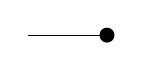
\begin{tikzpicture}
		\draw (0,0) node {} -- (-1,0);
	\end{tikzpicture}
	\caption{Vector \(\vec{a}\in\mathbb{R}^{n_1}\)}\label{fig:tnd:vec}
	\end{subfigure} ~
	\begin{subfigure}[t]{0.45\textwidth}
	\centering
	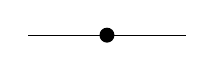
\begin{tikzpicture}
		\draw (1,0) -- (0,0) node {} -- (-1,0);
	\end{tikzpicture}
	\caption{Matrix \(\mat{B}\in\mathbb{R}^{n_1 \times n_2}\)}\label{fig:tnd:mat}
	\end{subfigure} \\
	
	\begin{subfigure}[t]{0.5\textwidth}
	\centering
	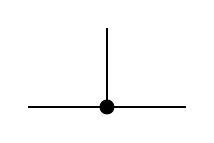
\begin{tikzpicture}
		\draw (0,0) node {}
			\foreach \x in {0,90,180}
			{
				(\x:1) -- (0,0)
			};
	\end{tikzpicture}
	\caption{Three-way tensor 
		\(\tensor{C}\in\mathbb{R}^{n_1\times n_2\times n_3}\)}\label{fig:tnd:3ten}
	\end{subfigure}
	\caption{Example tensor network diagrams.}
	\label{fig:tnegs}
\end{figure}

When \(\tensor{W}\) is a three-way tensor, we prefer a more compact notation
\begin{equation}\label{eq:bilintensor}
	\vec{z} = \tran{\vec{x}}\tensor{W}\vec{y}.
\end{equation} This loses none of the precision of the more verbose notation, provided we make clear
that we intend \(\vec{x}\) to operate along the first dimension of the tensor and \(\vec{y}\) the
third. That is to say, \((\tran{\vec{x}}\tensor{W})\vec{y}\) exactly corresponds with 
equation~\eqref{eq:bilinearkolda} while \(\tran{\vec{x}}(\tensor{W}\vec{y})\) corresponds to
equation~\eqref{eq:bilinearkolda2}. With either notation, for a tensor 
\(\tensor{W} \in \mathbb{R}^{n_1 \times n_2 \times n_3}\), we must have that 
\(\vec{x}\in \mathbb{R}^{n_1}\), \(\vec{y} \in \mathbb{R}^{n_3}\) and the result 
\(\vec{z}\in\mathbb{R}^{n_2}\).

An intuitive way to illustrate these ideas is using Tensor Network Diagrams
\autocite{Cichocki2016, Orus2014}. In these diagrams, each object is represented
as a circle, with each free `arm' representing an index used to address elements.
A vector therefore has one free arm, a matrix two and so on. Scalars will have
no arms. Figure~\ref{fig:tnegs} has examples for these simple objects. 

Where these diagrams are especially useful is for representing contractive products
where we sum over the range of a shared index. We represent this by joining the
respective arms. As an example, a matrix-vector product \(\vec{y} = \mat{Ax}\)
has such a contraction: \(y_{i} = \sum_{j}A_{ij}x_{j}\). This is shown in
figure~\ref{fig:tnmatvec} -- it is clear that there is only a single free arm, so the
result is a vector as it should be. Figure~\ref{fig:tnprods} shows some examples
of these kinds of products.

\begin{figure}
	\centering
	\begin{subfigure}[t]{0.45\textwidth}
		\centering
		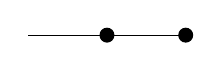
\begin{tikzpicture}
			\draw
				(1,0) node{} -- (0,0) node {} -- (-1,0);
		\end{tikzpicture}
		\caption{Matrix-vector product \(\mat{A}\vec{y}\), one free arm indicates
		 the result is a vector.}
		 \label{fig:tnmatvec}
	\end{subfigure} ~
	\begin{subfigure}[t]{0.45\textwidth}
		\centering
		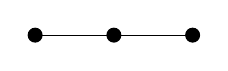
\begin{tikzpicture}
			\draw
				(1,0) node{} -- (0,0) node {} -- (-1,0) node{};
		\end{tikzpicture}
		\caption{Vector-matrix-vector bilinear form \(\tran{\vec{x}}\mat{A}
				 \vec{y}\). No free arms so the result is a scalar.}
	\end{subfigure}\\
	\begin{subfigure}[t]{0.45\textwidth}
		\centering
		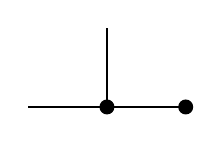
\begin{tikzpicture}
			\draw (0,0) node {}
				\foreach \x in {0,90,180}
				{
					(\x:1) -- (0,0)
				}
				(0:1) node{};
		\end{tikzpicture}
		\caption{Tensor-vector product produces a matrix.}
	\end{subfigure} ~
	\begin{subfigure}[t]{0.45\textwidth}
		\centering
		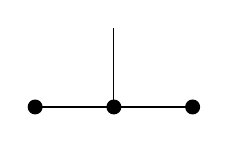
\begin{tikzpicture}
			\draw (0,0) node {}
				\foreach \x in {0,90,180}
				{
					(\x:1) -- (0,0)
				}
				(0:1) node{}
				(180:1) node{};
		\end{tikzpicture}
		\caption{Vector-tensor-vector product produces a vector.}
		\label{fig:vanillabilintnd}
	\end{subfigure}
	\caption{Various products expressed as Tensor Network Diagrams.}
	\label{fig:tnprods}
\end{figure}

\section{Bilinear Products}
There are several ways to describe the operation performed by the bilinear products we are
concerned with. These correspond to different interpretations of the results. The following
interpretations provide insight both into what is actually being calculated and how the product might
be applicable to a neural network setting. In all of the below we use the above definitions of
\(\vec{x}, \vec{y}, \vec{z}\) and \(\tensor{W}\).

\subsection{Interpretations}
\subsubsection{Stacked bilinear forms}
If we consider the expression for a single element of \(\vec{z}\), we get
\begin{equation} \label{eq:singlezsum}
	z_j = \sum_i^{n_1} \sum_k^{n_3} W_{ijk} x_i y_k
\end{equation} as expected. We can re-write this in terms of the slices of \(\tensor{W}\):
\begin{equation}\label{eq:singlezslice}
	z_j = \tran{\vec{x}}\tensor{W}_{\cdot j \cdot}\vec{y}
\end{equation} which reveals the motivation behind the notation in equation~\eqref{eq:bilintensor}.
It also reveals that each element of \(\vec{z}\) is itself linear in \(\vec{x}\) or \(\vec{y}\) if
the other is held constant.

This provides an interpretation
in terms of similarities. If we consider the standard dot product of two vectors 
\(\vec{a}\) and
\(\vec{b}\) of size \(m\): 
\begin{equation}
\langle\vec{a}, \vec{b}\rangle = 
\vec{a}^\mathsf{T}\vec{b}
= \sum_{i=1}^ma_ib_i
 = {\cos\theta}{||\vec{a}||_2||\vec{b}||_2} 
\end{equation} where
\(\theta\) is the angle in the angle between the vectors. If the product
is positive, the two vectors are pointing in a similar direction and if it is negative they
are in opposite directions. If it is exactly zero, they must be orthogonal. The dot product
therefore provides us with some notion of the similarity between two vectors.
Indeed if we normalise the vectors by dividing each component by their \(l_2\) norm we
recover exactly the widely used cosine similarity, common in information retrieval 
\autocite{Singhal2001, Tan2006} . Note that
we can generalise this idea by inserting a matrix of (potentially learned)
weights \(\mat{U}\) which enables us
to define general scalar bilinear forms
\begin{equation}
	\langle\vec{a}, \mat{U}\vec{b}\rangle = \langle\vec{a}^\mathsf{T}\mat{U}, \vec{b}\rangle
	= \vec{a}^\mathsf{T}\mat{U}\vec{b}.
\end{equation}

In a bilinear tensor product, each component of the result takes this form.
We can therefore think of the
product as computing a series of distinct similarity measures between the two input
vectors. With this in mind the obvious question is: what is the role of the matrix? The first
thing to note is that inserting a matrix into the inner product allows the two vectors to be
of different dimension. We also observe that a matrix-vector multiplication consists of
taking the dot product of the vector with each row or column of the matrix. Given our current
interpretation of the dot product as an un-normalised similarity measure, we can also
interpret a matrix-vector multiplication as computing the similarity of the vector with each
row or column of the matrix. 

We can then think of the rows of the matrix \(\mat{U}\) in the
above as containing patterns to look for in the \(\vec{b}\) vector and the columns to
contain patterns to test for in the \(\vec{a}\) vector. If we consider the vectors 
\(\vec{a}\) and \(\vec{b}\) to come from different feature spaces, the matrix \(\mat{U}\)
provides a conversion between them allowing us to directly compare the two. We can then
interpret each coordinate of the result of the bilinear tensor product as being an
independent similarity measure based on different interpretations of the underlying
feature space. In this sense, where a matrix multiplication looks for patterns in a single input
space, a bilinear product looks for \emph{joint} patterns in the combined input spaces of
\(\vec{x}\) and \(\vec{y}\).


\subsubsection{Choosing a matrix}
Following on from the above discussion we claim that for each coordinate of the output we are
computing a \emph{similarity vector} which we compare to the remaining input to generate a
scalar value. If we consider all coordinates at once, we see that this amounts to having
one input choose a matrix, which we then multiply by the remaining input vector. We have
refrained from making these points in terms of the specific vectors referenced above to make
the point that the operation is completely symmetrical. While it aids interpretation to think
of one vector choosing a matrix for the other vector, we can always achieve the same
intuition after switching the vectors, give or take some transposes.

This interpretation is very clear from the expression of the product in
equation~\\eqref{eqref{eq:bilinearkolda}. Simply by inserting parentheses we observe that we are
first generating a matrix in a way somehow dependent on the first input and multiplying
the second input by that matrix. In this sense we allow one input to choose patterns to look for
in the other input.

This intuition of choosing a matrix is suggested in \autocite{Sutskever2013} in the
context language modelling with RNNs. It is suggested that allowing the current input
character to choose the hidden-to-hidden weights matrix should confer benefits. 
This intuition (and the factorisation of the implicit tensor) was put to use earlier in the context
of Conditional Restricted Boltzmann Machines \autocite{Taylor} which actively seek to model the
conditional dependencies between two types of input.

Although this provides a powerful insight into the bilinear product, it is worth reinforcing that
the product is entirely symmetrical. We can not think purely about it as \(\vec{x}\) choosing a matrix
for \(\vec{y}\) as the converse is equally true.

\subsubsection{Tensor as an independent basis}
Extending the above to try and capture the symmetricity of the operation, we introduce
the notion that the coefficients of the tensor represent a basis in which to compare the
two inputs, independent of both of them. This idea is mentioned in
 \autocite{Tenenbaum2000} which considered the problem of data that can be described by two
independent factors.
The tensor then contains a basis which characterises the interaction by which the factors
in the input vectors combine to create an output observation.

This is a somewhat abstract interpretation -- to attempt to create a more concrete
 intuition
consider the case when both vectors have a single element set to \(1\) and the remainder
\(0\). In this case the first tensor-vector product corresponds to taking a slice of the
tensor, resulting in a matrix. The final matrix-vector product corresponds to picking a
row or column of the matrix. Consequently the whole operation is precisely looking up
a fibre of the tensor. To generalise from such a ``one-hot'' encoding of the inputs
to vectors of real coefficients, we simply replace the idea of a
\emph{lookup} with that of a \emph{linear combination}. The vectors then represent the coefficients
of weighted sums; first over slices and then over rows or columns. The final product is then a
distinct representation of both vectors in terms of the independent basis expressed by the tensor.

\subsubsection{Operation on the outer product}
n this section we describe the bilinear tensor product as operating on pairwise
products of inputs. This interpretation is essential for understanding the expressive
power of the operation as it gives rise to an obvious XOR-like behaviour. It also serves
as a useful reminder that a bilinear form is linear in each input only when the other
is held constant -- when both are allowed to vary we can represent complex non-linear
relations.
A way to approach this interpretation arises from a method of implementing the bilinear 
product in terms of straightforward matrix operations.

To discuss
this we introduce the notion of the \emph{matricisation} of a tensor. Intuitively this
operation is a way of \emph{unfolding} or \emph{flattening} a tensor into a matrix,
preserving its elements. Specifically the mode-\(n\)
matricisation of a tensor is defined as an operation which takes all mode-\(n\) fibres
of the tensor and places them as columns to create a matrix. We denote an mode-\(n\)
matricisation of a tensor \(\tensor{W}\) as \(\matr_n(\tensor{W})\). While the operation is
fairly straightforward, describing the exact permutation of the indices is awkard -- 
for a robust treatment of the general case (and the source of the above definition) see
\autocite{Kolda2009}. 

Although this notion captures and generalises the vectorisation operator often
encountered in linear algebra, we retain the classical \(\vect\) operator for clarity.
This flattens a matrix into a vector by stacking its columns. For some matrix \(\mat{A}\) with
\(n\) columns:
\begin{equation}\label{eq:vec}
	\vect(\mat{A}) = \begin{bmatrix}
		\vec{A}_{\midbullet 1}\\
		\vec{A}_{\midbullet 2}\\
		\vdots\\
		\vec{A}_{\midbullet n}
	\end{bmatrix}.
\end{equation}

For our purposes is is sufficient to note that a 
mode-2 matricisation of a
three-way tensor \(\tensor{W} \in \mathbb{R}^{n_1\times n_2\times n_3}\) must have shape
\(n_2 \times n_1n_3\). This gives us the following lemma, which shifts this line of
thinking slightly sideways.

\begin{lem}[Matricisation/vectorisation]
The \(j\)-th row of the mode-2 matricisation of the three-way tensor \(\tensor{W}\)
is equivalent to the vectorisation of the slice formed by fixing the second index at \(j\):
\begin{equation}\label{eq:matlemstatement}
	\matr_2 (\tensor{W})_{j \midbullet} = \vect(\mat{W}_{\midbullet j \midbullet}).
\end{equation}
\label{lem:matricise}
\end{lem}
\begin{proof}
By the above definition of the vectorisation operator, each index \((i, k)\) in some matrix
\(\mat{U} \in \mathbb{R}^{n_1\times n_3}\) maps to element \(i + (k-1)n_1\) in
\(\vect(\mat{U})\). By the definition of the mode-2 matricisation we would expect to
find tensor element \(W_{ijk}\) at index \((j, i + (k-1)n_3)\). Hence if we fix \(j\), we have
precisely the vectorisation of the \(j\)-th slice of the tensor.

The indices into \(\matr_2(\tensor{W})\) can be though of as arising from the following construction
process: first fix all indices to 1. Construct a column by sweeping the second index, \(j\),
through its full range. Then increment the first index \(i\) and repeat the procedure, placing
the generated columns with index \(i\). Only when \(i\) has swept through its full range
increment the final index \(k\) and repeat the procedure. The generated columns should then be
at positions \(i + (k-1)n_1\).
\end{proof}

These flattenings are important as they allow us to
implement many operations involving tensors in terms of a small number of larger matrix
operations when compared to the naive approach.

\begin{lem}[Matricised product]\label{lem:outerprod}
For a tensor \(\tensor{W}\) and vectors \(\vec{x}, \vec{y}\) as above,
we can describe the product \(\vec{z} = \tran{\vec{x}}\tensor{W}\vec{y}\) in terms of the
mode-2 matricisation of \(\tensor{W}\) as 
follows:
\begin{align}
	\vec{z} = \matr_2(\tensor{W})\mathrm{vec}\left[\vec{y}\tran{\vec{x}}\right]
	\label{eq:bilinearouter}
\end{align}
\end{lem}

\begin{proof}
To
prove this we can compare the expressions for a single element of the result.
An element \(z_j\) from equation~\eqref{eq:bilinearouter}
is formed as the inner product of the \(j\)-th
row of the flattened tensor and the vectorised outer product of the inputs. By 
lemma~\ref{lem:matricise}:
\begin{equation}
	z_j = 
	\sum_{s=1}^{n_1n_3} (\matr(\tensor{W})_{js} 
	\left( \vect\left[\vec{y}\vec{x}^\mathsf{T}\right]\right)_s
\end{equation}
We replace the sum over \(s\) with a sum over two
indices, \(i\) and \(k\), and using them to appropriately re-index the flattenings 
as described in lemma~\ref{lem:matricise} we 
derive
\begin{align}
	z_j &= \sum_{i=1}^{n_1}\sum_{k=1}^{n_3} W_{ijk} x_i y_k \\
		&= \tran{\vec{x}}\mat{W}_{\midbullet j \midbullet}\vec{y}
\end{align}

\end{proof}


Therefore to understand the bilinear product it helps to understand the matrix 
\(\vec{y}\vec{x}^\mathsf{T}\). Each element is of the following form:
\begin{equation}
	(\vec{y}\vec{x}^\mathsf{T})_{ki} = x_iy_k,
\end{equation} it contains all possible products of pairs of elements, one from each vector. 
This captures some interesting interactions.

\begin{thm} [Bilinear exclusive-or] \label{thm:xor}
Bilinear tensor products operate on the pair-wise exclusive-or of the
signs of the inputs.
\end{thm}
\begin{proof}
Consider the sign of a scalar product
\(c = a\cdot b\). If one of the operands \(a\) or \(b\) is positive and the other negative,
then the sign of \(c\) is negative. If both are positive or both are negative, then the
result is positive. This captures precisely the ``one or the other but not both'' structure
of the exclusive-or operation.

By lemma~\ref{lem:outerprod} a bilinear product can be viewed as a matrix operation on the flattened
outer product of the two inputs. As each element in the outer product is the product of two scalars,
the signs have an exclusive-or structure.
\end{proof}

\begin{cor}[Bilinear conjunctions]\label{cor:and}
If the inputs are binary, bilinear products operate on pair-wise conjunctions of the inputs.
\end{cor}
\begin{proof}
If \(a, b \in \{0, 1\}\), then \(a \cdot b = 1\) if and only if both \(a\) and \(b\) are \(1\). If
either or both are \(0\) then their product must be zero. Following the same structure as the proof
of theorem~\ref{thm:xor}, for binary inputs we must have this conjunctive relationship.
\end{proof}

\subsubsection{Remarks on theorem~\ref{thm:xor}}
There are a number of remarks worth making about these results. Firstly they suggest considering
the case where both inputs are the same: \(\vec{z} = \tran{\vec{x}}\tensor{W}\vec{x}\). Replacing
bilinear forms with quadratic forms may invalidate some of the similarity based interpretations,
but it might also provide an interesting class of very powerful feed-forward networks. As an example,
note that a plain perceptron has been long known to be incapable of learning the exclusive-or
mapping \autocite{Minsky1969} -- a neural network to solve the problem requires either a hidden layer
or an additional input feature (specifically the conjunction of the inputs) \autocite{Rumelhart1986}.
By corollary~\ref{cor:and} this quadratic tensor form would implicitly and naturally capture the
additional conjunctive feature and be capable of solving the exclusive or problem without hidden
layers or hand-engineered features.

Secondly, this captures the notion that the bilinear tensor product operates implicitly on higher
level features, constructed by combining both inputs. This indicates that it is capable of capturing
complex relationships between the two inputs.

Finally we will point out that this gives an indication of what we term the `apparent depth' of the
tensor product. While it has long been known that neural networks with a single hidden layer and
appropriate non-linearity (and therefore two weight matrices)
 are universal function approximators \autocite{Hornik1989}, recent results
have suggested that the depth of the network is important in keeping the number of parameters
bounded \autocite{Eldan2016, Telgarsky2016}. In particular, Eldan and Shamir show that for a
particular class of radial basis-like functions (which depend only on the squared norm of the input)
there exist networks with two hidden layers and a number of nodes polynomial in the input dimension
which can perfectly approximate the function. They then show that a shallower network with a single
hidden layer can only perfectly approximate the function with a number of nodes exponential in the
input dimension \autocite{Eldan2016}.

Eldan and Shamir's proof constructs a three-layer network in the following manner:
for an input \(\vec{x}\), the first two layers learn to approximate the map 
\(\vec{x}\to ||x||^2_2 = \sum_i x_i^2\) while the final layer learns a univariate function on the
squared norm \autocite{Eldan2016}.
 
It is straightforward to see that a quadratic tensor layer as discussed above could compute the
squared norm. Consider the product \(\tran{\vec{x}}\tensor{W}\vec{x}\) and let 
\(\tensor{W} = [\mat{A},\mat{B},\mat{C}]_{CP}\) be represented in the CP-decomposition with
rank \(d\), where \(d\) is also the size of the inputs. Then if we let 
\(\mat{A}=\mat{C}=\mat{I}_d\) and \(\mat{B}\) be a \(d \times 1\) vector of ones,
we have
\begin{align}
	\tran{\vec{x}}\tensor{W}\vec{x} 
	&= \tran{\mat{B}}\left(\mat{A}\vec{x} \odot \mat{C}\vec{x}\right)\\
	&= \tran{\vec{1}}(\vec{x} \odot \vec{x})\\
	&= \sum_{i=1}^d x_i^2 = ||\vec{x}||^2_2.
\end{align} Thus we can compute the squared norm with only a single tensor layer, while it requires
two standard layers. This is a useful intuition: using tensors in a neural network allows us to
limit the number of hidden layers while maintaining much of the expressive power and polynomial
parameters.

\section{Tensor Decompositions}
The ultimate goal is to learn the tensor that parameterises a bilinear product. Unfortunately
such a tensor is often very large; an \(n \times n \times n\) would require \(O(n^3)\) space
to store explicitly. Further,
it is highly likely that we will be looking to model simpler interactions than the full tensor
might represent. This leads to the idea of a parameterised decomposition -- an ideal solution
would be a method of representing the tensor with some way of specifying the complexity of the
bilinear relationship and hence making explicit the relationship between the number of parameters
required and the expressive power of the model. 

We will investigate two methods of tensor decomposition with a view towards their use as a building
block for neural networks. The outcomes we wish to evaluate are: the savings in storage, how
convenient it is to specify the number of parameters, convenience and efficiency of implementation
(in terms of matrix operations) and whether the gradients suggest any benefits or hindrances when
learning by gradient descent. There is a significant amount of research into tensor decompositions,
\autocite{Kolda2009} provides a thorough review. Here we consider some of the most general
decompositions and families of decompositions without going into detail outside of where it is
relevant to the above concerns.

\subsection{CANDECOMP/PARAFAC}
This method of decomposing a tensor dates as far back as 1927 
\autocite{Hitchcock1927, Hitchcock1928} and was rediscovered repeatedly across a range of
communities over the next 50 years \autocite{Kolda2009}. First referred to as `polyadic
form of a tensor' we refer to it as the CP-decomposition after two prominent publications in
1970 referring to the technique as `canonical decomposition' (CANDECOMP) \autocite{Carroll1970}
 or `parallel factors' (PARAFAC) \autocite{Harshman1970}. 
 It is a fairly straightforward
extension of a matrix rank decomposition to the more general case, representing a tensor as
a sum of rank one tensors. This section contains a formal description of the three-way case
as well as a note on computing bilinear products with the decomposed tensor.
Some interesting results on the uniqueness of the decompositions can be found in \autocite{Kolda2009},
but they are not relevant to the discussion here.

\subsubsection{Description}
Given a three-way tensor \(\tensor{X} \in \mathbb{R}^{n_1 \times n_2 \times n_3}\) we wish to 
approximate it as
\begin{equation}\label{eq:cp-statement}
	\tensor{X} \approx \sum_{r=1}^{R} \vec{a}_r \otimes \vec{b}_r \otimes \vec{c}_r
\end{equation}
 where \(R\) is the rank of the decomposition and \(\cdot \otimes \cdot\) denotes the tensor
product. This product expands the dimensions; for the first two vectors it is the outer product
\(\vec{a}\tran{\vec{b}}\) which generates a matrix consisting of the product of each pair of
elements in \(\vec{a}\) and \(\vec{b}\). With three such products we proceed analogously, except
now our structure must contain the product of each possible triple of elements. Hence we need
three indices to address each entry, so it best described as a three-way tensor. Each individual
element has the form
\begin{equation}\label{eq:cp-element}
	X_{ijk} = \sum_{r=1}^R a_{ri}b_{rj}c_{rk}.
\end{equation}

It is convenient to stack these factors into matrices --
we differ slightly from \autocite{Kolda2009} by defining the \textit{factor matrices} of the 
form \(\mat{A} = [\vec{a}_1\;\vec{a}_2\;\cdots\;\vec{a}_R]^{\mathsf{T}} \in 
\mathbb{R}^{R\times n_1}\) (and equivalently for
\(\mat{B}\) and \(\mat{C}\)) such that the  \textit{rows} of the matrix correspond to the
\(R\) vectors. 
We denote a tensor decomposed in this format 
\(\tensor{X} = [\mat{A}, \mat{B}, \mat{C}]_{CP}\).

\subsubsection{Bilinear Product}
We wish to compute a product of the form \(\vec{z} = \tran{\vec{x}}\tensor{W}\vec{y}\)
where \(\tensor{W} = [\mat{A}, \mat{B}, \mat{C}]_{CP}\) is represented as a CP-decomposition.
Conveniently, this can be done with simple matrix products.

\begin{prop} \label{prop:cpbilin}
\begin{align}
	\vec{z} &= \tran{\vec{x}}\tensor{W}\vec{y} \\
			&= \tran{\mat{B}}(\mat{A}\vec{x} \odot \mat{C}\vec{y})
\end{align}
when \(\tensor{W} = [\mat{A}, \mat{B}, \mat{C}]_{CP}\) and \(\odot\) represents the Hadamard
(elementwise) product.
\end{prop}
\begin{proof}
This follows from straightforward rearranging. Firstly
\begin{align}
	z_j &= \sum_{i}^{n_1} \sum_k^{n_3} W_{ijk} x_i y_k \\
		&= \sum_{i}^{n_1} \sum_k^{n_3} \sum_r^R A_{ri} B_{rj} C_{rk} x_i y_k\\\label{eq:cpbilin-one}
		&= \sum_r^R B_{rj} \left( \sum_i^{n_1} A_{ri} x_i \cdot \sum_k^{n_3} C_{rk}y_k \right).
\end{align}
This implies we can compute the quantity inside the brackets for all \(r\) at once simply
by \(\mat{A}\vec{x} \odot \mat{C}\vec{y}\) which results in a length \(R\) vector. 
Equation~\eqref{eq:cpbilin-one} then notes that for each output \(j\) we take the \(j\)-th column
of the \(R \times n_2\) factor matrix \(\mat{B}\) and perform a dot product with our earlier
result. A series of dot products can be easily expressed with matrix multiplication, noting
that we have to transpose \(\mat{B}\) to keep it on the left but still sum over each column.
Hence:
\begin{equation}
	\vec{z} = \mat{B}^\mathsf{T} (\mat{A}\vec{x} \odot \mat{C}\vec{y}).
\end{equation}
\end{proof}

We can express the bilinear product above as a tensor network diagram, although we have to insert
an auxiliary \(R\times R\times R\) tensor, denoted \(\tensor{I}_{R}\) which is defined as
\begin{equation}\label{eq:tensoridentity}
	I_{ijk} = \begin{cases}
		1 & \mathrm{if} \; i=j=k \\
		0 & \mathrm{otherwise}
	\end{cases}
\end{equation} in a manner analogous to the identity matrix. Taking a bilinear product with this
tensor simply represents elementwise multiplication of the two vectors. In the diagram this is
represented with the symbol
\rotatebox[origin=c]{-180}{\(\oslash\)} to emphasise the diagonality (and to emphasise that it
it is different as we do not need to store its parameters).
This is presented in 
figure~\ref{fig:cpbilintnd}, which can be compared to figure~\ref{fig:vanillabilintnd}.

\begin{figure}
	\centering
		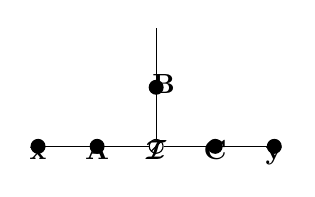
\begin{tikzpicture}[scale=0.75]
			\node (0,0) [forbidden sign, 
						 rotate=180, 
						 draw, fill=none, label=above:{\(\tensor{I}\)}] (I) {};
			\draw
				(-2,0) node[label=below:{\(\vec{x}\)}]{}
				 -- (-1,0) node[label=below:{\(\mat{A}\)}]{}
				 -- (I)
				(2,0) node[label=below:{\(\vec{y}\)}]{}
				 -- (1,0) node[label=below:{\(\mat{C}\)}]{}
				 -- (I)
				(I) --
				(0,1) node[label=right:{\(\mat{B}\)}]{}
				 -- (0,2)
			;
		\end{tikzpicture}
	\caption{One way of representing a bilinear product in the CP-decomposition.}
	\label{fig:cpbilintnd}
\end{figure}


\subsubsection{Gradients}
As the final aim is to attempt to learn the coefficients of the decomposition using gradient
descent, it makes sense to check that the gradients of the parameters are well-behaved
with respect to the output of the bilinear product. We break the gradient into three parts,
one for each of the parameter matrices. \hl{do this properly}

Let \(\vec{z}\) be defined as above.
The gradient of \(\vec{z}\) with respect to \(\mat{A}\) has entries of the form:
\begin{align}
	\frac{\partial z_j}{\partial A_{lm}} &= x_m \cdot \sum_k^{n_3}C_{lk}y_k \\
		&= x_m \cdot \vec{C}_{l\midbullet}^\mathsf{T}\vec{y}.\\
\intertext{The gradients with respect to \(\mat{C}\) have the same form:}
	\frac{\partial z_j}{\partial C_{lm}} &= y_m \cdot \sum_i^{n_1}A_{li}x_i \\
		&= y_m \cdot \vec{A}_{l\midbullet}^\mathsf{T}\vec{x}.\\
\intertext{The gradient of the final parameter matrix \(\mat{B}\) has entries}
	\frac{\partial z_j}{\partial B_{lm}} &= 
		\mathbb{I}_{m = j} \cdot \left( \mat{A}\vec{x} \odot \mat{C}\vec{y}\right)
\end{align} where \(\mathbb{I}_{m=j}\) denotes the indicator function that is one if
\(i = j\) and zero otherwise.
This has the
curious effect that the gradient of the product with respect to \(\mat{B}\) is the same for all
columns of \(\mat{B}\). While this seems like it may hinder learning, in practice there
will be additional terms due to the loss function which ameliorate this.


\subsubsection{Storage Requirements}
The number of stored coefficients for a rank \(R\) CP-decomposed tensor of size 
\(I \times J \times K\) will be \(RI + RJ + JK\). Explicitly storing the tensor would require
\(IJK\) numbers to be stored. To illustrate the significance of this, consider the case when
the tensor being decomposed has all dimensions and rank of equal size. Denoting the size as
\(I\), then the explicit tensor will have an \(I^3\) storage requirement while the decomposed
tensor needs only \(3I^2\).


\subsection{Tensor Train, Tucker}
The \emph{tensor-train} decomposition has a much shorter history -- it was first proposed in
2011 as a simpler way of representing a slightly hierarchical form derived from a
generalisation of the singular value decomposition \autocite{Osedelets2011}. It is proposed
as an alternative to the CP-decomposition which purportedly provides benefits in terms of
numerical stability. It has been used to learn compressed weight matrices in large neural
networks \autocite{Novikov} suggesting it is a prime candidate to learn with gradient descent.
In the three-way case it is nearly equivalent to the more venerable Tucker decomposition
\autocite{Tucker1966}. The tensor train turns out to be simpler so beyond showing the similarity,
we consider primarily the tensor train.

It is also important to note that the tensor-train can be used more creatively. In \autocite{Novikov}
Novikov et al. use the decomposition to compress the final layers of a large convolutional neural
network by reshaping the matrices into high dimensional tensors. The reduction in parameters for
the tensor-train is most notable with particularly high-dimensional tensors, so this approach allows
for significant compression. They also show methods of computing the required matrix vector products
without having to expand the tensor. While this approach is highly successful, the implementation
(especially of back-propagation) is somewhat involved and it admits a very large number of ways of
applying the decomposition. To keep our search space of decompositions feasible, we limit to standard
application of the tensor-train.

\subsubsection{Description}
The tensor-train decomposition (TT-decomposition) of a general tensor \(\tensor{X}\) with
\(d\) indices is the tensor \(\tensor{Y} \approx\tensor{X}\) with elements expressed as a
product of slices of three-way tensors (so a product of matrices):
\begin{equation}
			\label{eq:tensortrain_full}
	{Y}_{i_1i_2\dots i_d} 
		= \mat{G}[1]_{\midbullet i_1 \midbullet}\mat{G}[2]_{\midbullet i_2 \midbullet}
			\cdots \mat{G}[d]_{\midbullet i_d \midbullet}.
\end{equation}
If dimension \(j\) is of size \(n_j\), then \(\tensor{G}[j]\) is size 
\(r_{j-1} \times n_j \times r_{j}\) so that each slice \(\mat{G}[j]_{\midbullet i \midbullet}\)
is size \(r_{j-1} \times r_{j}\). The collection of \(r_i\) is the `tt-rank' of the
decomposition and controls the number of parameters. In order to make the result of the chain
of matrix products a scalar, we have to ensure \(r_0 = r_d = 1\) \autocite{Osedelets2011}.

The three-way case presents no obvious simplifications from the general case but we present it
here to ensure consistent notation through the remainder of this section. The TT-decomposition
of a three-way tensor of size \(n_1 \times n_2 \times n_3\) has three `cores' with shapes
\(1 \times n_1 \times r_1\), \(r_1 \times n_2 \times r_2\) and \(r_2 \times n_3 \times 1\). For
convenience, we can treat these as a matrix, a three-way tensor and a matrix by ignoring 
dimensions of size one. This leads to the following expression of 
equation~\ref{eq:tensortrain_full} where \(\tensor{W}\) is the three way tensor in its
decomposed form:
\begin{equation} \label{eq:tensortrain_three}
	W_{ijk} = \mat{A}_{i\midbullet} \mat{B}_{\midbullet j \midbullet} \mat{C}_{\midbullet k}.
\end{equation} In a manner consistent with the CP-decomposition we denote such a decomposed
tensor \(\tensor{W} = [\mat{A},\tensor{B},\mat{C}]_{TT}\). It is important to note that the
shapes are less consistent: \(\mat{A}\) is an \(n_1 \times r_1\) matrix, \(\tensor{B}\) a
\(r_1 \times n_2 \times r_1\) tensor and \(\mat{C}\) an \(r_2 \times n_3\) matrix.

As this decomposition only contains contractive products, it is very well expressed as a Tensor
Network diagram. Figure~\ref{fig:tttnds} shows both the general case and the three-way case --
the general case shows clearly how we can build a tensor with a large number of dimensions purely
out of relatively small three-way tensors. The Tucker decomposition is also presented to illustrate
the similarities in the three-way case. It is also worth contrasting with figure~\ref{cp:bilintnd}
to see how the CP-decomposition can arise as a special case, a notion which is formalised later.

\begin{figure}
	\centering
	\begin{subfigure}[t]{0.45\textwidth}
		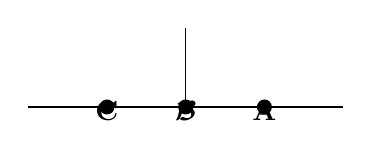
\begin{tikzpicture}
		\draw
				(2,0) -- (1,0) node[label=below:{\(\mat{A}\)}]{}
				-- (0,0)
				(-2,0) -- (-1,0) node[label=below:{\(\mat{C}\)}]{}
				-- (0,0)
				(0,0) node[label=below:{\(\tensor{B}\)}]{} -- (0,1)
			;
		\end{tikzpicture}
		\caption{Three-way tensor train.}
	\end{subfigure}~
	\begin{subfigure}[t]{0.45\textwidth}
		\begin{tikzpicture}
		\draw
				(2,0) -- (1,0) node[label=below:{\(\mat{C}\)}]{}
				-- (0,0)
				(-2,0) -- (-1,0) node[label=below:{\(\mat{A}\)}]{}
				-- (0,0)
				(0,0) node[label=below:{\(\tensor{B}\)}]{} -- (0,1)
				-- (0,1) node[label=right:{\(\mat{C}\)}]{} -- (0,2)
			;
		\end{tikzpicture}
		\caption{Three-way Tucker decomposition.}
		\label{fig:tuckertnd}
	\end{subfigure}\\
	\begin{subfigure}[t]{0.45\textwidth}
		\begin{tikzpicture}
		\draw
				(-2,0) -- (-1,0) node{}
				-- (0,0) node{} -- (0,1)
				(-1,0) -- (-1, 1)
				(0,0) -- (0,1)
				(0,0) -- (1,0)
				
				(2,0) -- (3,0) node{}
				-- (4,0)
				(3,0) -- (3, 1)
			;
		\path (1,0) -- node[auto=false, draw=none, fill=none] {\ldots} (2,0);
		\end{tikzpicture}
		\caption{General Tensor Train}
	\end{subfigure}
	\caption{Diagrams of the Tensor Train and Tucker decompositions.}
	\label{fig:tttnds}
\end{figure}

\subsubsection{Bilinear Product}
Computing a bilinear product between two vectors and a tensor in the TT-decomposition does not
have quite such an efficient form as the CP-decomposition. Primarily this is due to the presence
of the three-way tensor \(\tensor{B}\), which means we are still eventually computing a full
tensor product, simply with a smaller tensor. We denote the product as
\begin{equation} \label{eq:tt_bilin}
	\vec{z} = \vec{x}^\mathsf{T}\mat{A}\tensor{B}\mat{C}\vec{y}.
\end{equation} For a specific index this has the form
\begin{align} \label{eq:tt_bilin_index}
	z_j &= \vec{x}^\mathsf{T}\vec{A}\mat{B}_{\midbullet j \midbullet}\mat{C}\vec{y}\\
		&= \sum_{i=1}^{I}\sum_{k=1}^K\sum_{m=1}^{r_1}\sum_{n=1}^{r_2}A_{im}B_{mjn}C_{nk}x_iy_k.
\end{align}

This provides a clear intuition about what the TT-decomposition is doing in the three-way case.
Matrices \(\mat{A}\) and \(\mat{C}\) project the inputs into a new (potentially smaller) space
where the bilinear product is carried out with \(\tensor{B}\) ensuring the result has been pushed
back to the appropriate size.


\subsubsection{Gradients}
\hl{Should do all at once?}
In the TT-decomposition the gradients are very similar.
The gradient of \(\vec{z}\) with respect to \(\mat{A}\) has entries of the form:
\begin{align}
	\frac{\partial z_j}{\partial A_{lm}} 
		&= x_l \cdot \left(\vec{B}_{mj\midbullet}^\mathsf{T}\mat{C}\vec{y}\right). \\
\intertext{The components of the gradient with respect to \(\mat{C}\) have a similar form:}
	\frac{\partial z_j}{\partial C_{ml}} 
		&= y_l \cdot \left(\vec{B}_{\midbullet jm}^\mathsf{T}\mat{A}\vec{x}\right). \\
\intertext{While the gradient of the elements of \(\tensor{B}\) behave surprisingly similarly
	to the CP-decomposition:}
	\frac{\partial z_j}{\partial B_{lmn}} 
		&= \mathbb{I}_{m = j} \cdot \left( \mat{A}\vec{x} \odot \mat{C}\vec{y}\right).
\end{align}


\subsection{Comparison}
In this section we first prove a result on the conditions required for the decompositions to
be equivalent. This is followed by a brief discussion of the theoretical differences and
similarities between the two decompositions and whether we can draw any conclusions about their
suitability for the task at hand. 

It is also worth noting briefly that the gradients are very nearly equivalent. This implies
that attempting to learn the parameters directly using gradient descent should work for both
or neither, since it seems reasonable to expect similar dynamics.

\subsubsection{Equivalence}
One condition for the tensor-train to be equivalent to the CP-decomposition is if the central
tensor in the TT-decomposition has diagonal, square slices. Intuitively this reduces the tensor
product to a matrix product. 

\begin{prop}
The rank \(R\) CP-decomposition of a tensor \(\tensor{X} = [\mat{A},\mat{B},\mat{C}]_{CP}\) is
equivalent to a TT-decomposition \([\mat{A}', \tensor{B}', \mat{C}']_{TT}\) with both ranks
equal to \(R\) and \(\tensor{B}'_{ijk} = 0\) except where \(i=k\).
\end{prop}
\begin{proof}
Consider the slices of \(\tensor{X} \in \mathbb{R}^{n_1 \times n_2 \times n_3}\) formed by fixing the
second index and allowing the first and third to vary. If 
\(\tensor{X} = [\mat{A}, \mat{B}, \mat{C}]_{CP}\) then these slices can be expressed concisely as
\begin{equation} \label{eq:cp-slice}
	\mat{X}_{\midbullet j \midbullet} = \mat{A}\diag({\mat{B}_{j\midbullet}})\tran{\mat{C}}
\end{equation} where \(\diag(\vec{v})\) denotes the matrix with vector \(\vec{v}\) along the
leading diagonal and zero elsewhere. In the above the vector is in fact the \(j\)-th row of
the factor matrix \(\mat{B}\). It is clear the the diagonal matrix must then have shape
\(R \times R\) so the result has the expected shape \(n_1 \times n_3\). We also verify this gives us
the appropriate expression for a single element of the tensor:
\begin{align}
	X_{ijk} &= \left(\mat{A}\diag({\mat{B}_{j\midbullet}})\tran{\mat{C}}\right)_{ik} \\
		    &= \sum_{\alpha=1}^R A_{i\alpha} \cdot
		    	\left(\sum_{\beta=1}^{R} \diag(B_{j\midbullet})_{\alpha\beta} C_{k\beta}\right) \\
			&= \sum_{\alpha=1}^R A_{i\alpha} B_{j\alpha} C_{k\alpha}
\end{align} where the last step follows from diagonality.

We now construct a TT-decomposition \(\tensor{X} = [\mat{A}', \tensor{B}', \mat{C}']_{TT}\)
of the same tensor. The ranks of the decomposition will be \(r_1 = r_2 = R\) for \(R\) the rank
of the corresponding CP-decomposition.
Let \(\mat{A}' = \mat{A}\) and \(\mat{C}' = \tran{\mat{C}}\). Construct tensor \(\tensor{B}'\)
by
\begin{equation}
	B_{ijk}' = \begin{cases}
		B_{ij} & \text{if}\; i = k \\
		0    & \text{otherwise}.
	\end{cases}
\end{equation}

An expression for the central slices of \(\tensor{X}\) in terms of its TT-decomposition which
follows from the element-wise definition is
\begin{align}
	\mat{X}_{\midbullet j \midbullet} &= \mat{A}'\mat{B}_{\midbullet j \midbullet}'\mat{C}'\\
	&= \mat{A}\diag(B_{j\midbullet})\tran{\mat{C}}
\end{align}
by construction of \(\tensor{B}\).
\end{proof}

As is demonstrated in figure~\ref{fig:tuckertnd} the Tucker decomposition is very similar to the 
tensor-train in the three-way case. For brevity we refrain from presenting the full Tucker
decomposition -- it suffices to note that it has matrices for all three dimensions rather than
just two. In order to convert the Tucker decomposition to the tensor-train, it is enough to multiply
the additional matrix with the central tensor. For that reason, we prefer the simpler tensor-train.

\subsubsection{Space Requirements}
The CP-decomposition is appealing because it has a single hyper-parameter \(r\). Further, the
storage of a CP-decomposed tensor is linear in \(r\). By comparison the TT-decomposition has
two parameters and the total storage requirement grows linearly in their product. This makes
choosing the parameter potentially easier with the CP-decomposition. If we take the easy option
and set both ranks of the TT-decomposition to the same value, then the number of elements is
proportional to the square of that value. As the rank has to be an integer, this potentially gives
us fewer feasible options.

\section{Learning decompositions by gradient descent}
We now present some experimental results, with two aims in mind. Firstly, it is instructive to compare
the performance of the two tensor decompositions when learnt by gradient descent on some
straightforward tasks. Secondly we wish to verify that a tensor decomposition is capable of learning
complicated structure by applying it to a classic benchmark and a real world example.

\subsection{Random Bilinear Products}\label{sec:randbilin}
The first test uses the following procedure: generate a fixed random tensor \(\tensor{T}\)
in the chosen decomposition with rank \(r_T\). Then generate a second tensor \(\tensor{W}\) 
with rank \(r_W\). At each stage \(t\) generate a pair of random input vectors \(\vec{x}_t\) and
\(\vec{y}_t\) and compute the bilinear products 
\(\vec{z}_tt = \vec{x}_t^\mathsf{T}\tensor{T}\vec{y}_t\) and 
\(\hat{\vec{z}}_t = \vec{x}_t^\mathsf{T}\tensor{W}\vec{y}_t\). Finally update the parameters of
\(\tensor{W}\) to minimise the mean squared error between \(\vec{z}^t\) and \(\hat{\vec{z}}^t\)
using stochastic gradient descent. In this way we hope to learn an approximation to 
\(\tensor{T}\) in a similar setting to what might be found inside a neural network.

In practice it is computationally expedient to deal with more than one vector at a time, in
all of the results for this section we use a batch size of \(32\). We use a fairly aggressive
 learning rate of \(0.1\).
Training continues for \(250,000\) parameter updates, although most of the tensors have stopped
making significant improvements by that time. In all tests the input vectors had elements drawn
from a uniform distribution over the range \([-1,1]\) while unless otherwise noted the elements of
the decomposition are drawn from a normal distribution with mean \(0\) and standard deviation
\(0.1\).

The results of attempting to approximate a rank 100 tensor with dimensions 
\(100 \times 100 \times 100\) are shown in figure~\ref{fig:cpapprox} and are more or less
as anticipated when attempting to approximate a CP-decomposition with another CP-decomposition.
When the approximator is a TT-decomposition, it was found to be very difficult to achieve a
good approximation -- when the learning rate was dropped to account for the apparent high
sensitivity of the loss the still failed to approach the error rates of the CP-decomposition.
While we might expect the CP-decomposition to better represent another CP-decomposition due to
the shared structure, it is nonetheless remarkable how difficult the TT-decomposition was to
train.

In general we see that the quality of the approximation drops consistently with the
number of parameters in the approximator, which is to be expected. 
More unexpected is the variance apparent in the training
curves of the CP-decomposition -- the very low rank approximations seem more sensitive to small
 changes in their coefficients. This suggests that some care
may need to be taken with the learning rates and the initialisation especially in deeper models as
when such difficulties will be compounded.
It is also useful to note that over-specifying the rank of the decomposition
appears to still aid learning.


The experiment was repeated with the target tensor expressed is a TT-decomposition with ranks
\(r_1 = r_2 = 16\) (28,800 coefficients). Results can be seen in figure~\ref{fig:ttapprox}.
As should be expected, the TT-decomposition performed better. In particular a TT-decomposition
matching the rank of the target tensor reached a very low error extraordinarily quickly,
performing much better than the CP-decomposition under the same conditions.

These results imply both decompositions are potentially useful. The CP-decomposition seems to
be capable of learning reasonable approximations even when it does not necessarily reflect the
structure of the underlying problem. The TT-decomposition appears to struggle in this situation,
but when the problem is structured in a more favourable way it seems to take greater advantage.

\begin{figure}
\centering
\begin{subfigure}[t]{0.45\textwidth}
	\includegraphics[width=\textwidth]{tensors/cp100cpapprox}
	\caption{Attempting to approximate by directly learning factor matrices representing a 
		CP-decomposition of various ranks}
	\label{fig:cpcpapprox}
\end{subfigure}
~
\begin{subfigure}[t]{0.45\textwidth}
	\includegraphics[width=\textwidth]{tensors/cp100ttapprox}
	\caption{Attempting to approximate by directly learning a TT-decomposition of various ranks}
	\label{fig:cpttapprox}
\end{subfigure}
\caption{Results for learning direct approximations of a CP-rank 100 tensor.}
 \label{fig:cpapprox}
\end{figure}

\begin{figure}
\centering
\begin{subfigure}[t]{0.45\textwidth}
	\includegraphics[width=\textwidth]{tensors/tt16cpapprox}
	\caption{Attempting to approximate by directly learning a 
		CP-decomposition of various ranks}
	\label{fig:ttcpapprox}
\end{subfigure}
~
\begin{subfigure}[t]{0.45\textwidth}
	\includegraphics[width=\textwidth]{tensors/tt16ttapprox}
	\caption{Attempting to approximate by directly learning a TT-decomposition of various ranks}
	\label{fig:ttttapprox}
\end{subfigure}
\caption{Results for learning direct approximations of a tt-rank 16 tensor.}
\label{fig:ttapprox}
\end{figure}

\subsection{Learning to multiply}
Learning bilinear functions provides a way to linearly approximate functions of two variables.
A motivating example of such a function is elementwise multiplication, also known as the Hadamard
product. In this section we investigate briefly the ability of the two decompositions to model
such a product.

\subsubsection{Theory}
We wish to determine first how to construct a tensor that represents an elementwise product and
then determine the rank of the decomposition required to represent it. Note that the tensor must
have the same size in all dimensions as the inputs and
 output of the product must be the same size. This tensor must be \textit{diagonal} with the
 diagonal elements having value one
 (see proposition~\ref{prop:identity} in the appendix for a proof). This means all entries
\(ijk\) such that \(i = j = k\) must be one, all other entries zero. We denote such a tensor
by \(\tensor{H}\).

Now we consider how the two proposed decompositions could model this tensor. For the 
CP-decomposition this is straightforward:
\(\tensor{H} = [\mat{I}, \mat{I}, \mat{I}]_{CP}\) where \(\mat{I}\) is the 
\(N\times N\) identity matrix. This is can be easily verified as the definition of a bilinear
product with a CP-decomposed tensor includes an elementwise product so it suffices to ensure the
factor matrices do not alter the inputs. The CP-decomposition reduces the required parameters
to \(3N^2\) as opposed to the original \(N^3\). This is a remarkable reduction, considering that
an analogous diagonal \emph{matrix} is the worst case for the corresponding two-way 
decomposition. 

The TT-decomposition is not capable of reducing the parameters. In order to ensure that the
central tensor product passes through the appropriate elements it must in
fact be equal to \(\tensor{H}\) itself.

\subsubsection{Experiments}
Learning exact elementwise products is a special case and can clearly be done with the 
CP-decomposition without sacrificing parameter reduction. The question that remains is how closely
a given decomposition can approximate an elementwise product, especially if there is some kind of
helpful latent structure in the inputs to exploit. We test this by inducing a random structure
on the inputs.

First we verify our theories about the capacity of the decompositions to represent elementwise
multiplication. This is performed identically to the experiments in section~\ref{sec:randbilin}
except that that rather than generating a random tensor to provide the targets for training,
we simply multiply elementwise the input vectors. We also simplify slightly by drawing the
input vectors from \(\{0,1\}\) with equal probability
(elementwise multiply in this sense corresponds to a bitwise AND). 
Again the squared error loss is used, although
a momentum term (with coefficient 0.9) was found to greatly assist learning.
For a further test, the target
output has a fixed permutation applied which removes the diagonal structure from the target but
should still be a straightforward task. For this task we would
expect that the CP-decomposition drastically outperforms the TT-decomposition.

The results, figures~\ref{fig:multiply-ff} and \ref{fig:permute-multiply-ff}, affirm our
expectations. The CP-decomposition is able to consistently reduce error as rank increases
 while the TT-decomposition appears to struggle.


\begin{figure}
	\begin{subfigure}[t]{0.45\textwidth}
		\includegraphics[width=\textwidth]{tensors/multiply-cp-mom}
		\caption{Learning curves for CP-decompositions learning elementwise multiplication}
	\end{subfigure}
	~
	\begin{subfigure}[t]{0.45\textwidth}
		\includegraphics[width=\textwidth]{tensors/multiply-tt-mom}
		\caption{Learning curves for TT-decompositions learning elementwise multiplication}
	\end{subfigure}
	\caption{Training error for various rank decompositions on the elementwise multiplication
	task.}
	\label{fig:multiply-ff}
\end{figure}

\begin{figure}
	\begin{subfigure}[t]{0.45\textwidth}
		\includegraphics[width=\textwidth]{tensors/permute-cp-mom}
		\caption{Learning curves for CP-decompositions learning permuted 
		elementwise multiplication}
	\end{subfigure}
	~
	\begin{subfigure}[t]{0.45\textwidth}
		\includegraphics[width=\textwidth]{tensors/permute-tt-mom}
		\caption{Learning curves for TT-decompositions learning permuted
		 elementwise multiplication}
	\end{subfigure}
	\caption{Training error for various rank decompositions on the permuted
	elementwise multiplication
	task.}
	\label{fig:permute-multiply-ff}
\end{figure} 


For a more realistic test we introduce a random structure to the input vectors. This is done by
creating smaller vectors and expanding them to the appropriate size by copying the
elements to random positions. The mapping of positions is fixed for the duration of a training
run. We then experiment with varying the size of these smaller vectors and hence varying the
degree of correlation while keeping the rank of the decomposition fixed. Here we have fewer
preconceptions regarding the relative performance of the decompositions.


The results again show the CP-decomposition outperforming the TT-decomposition dramatically.
In this case this is slightly more surprising as there is more likely to be solutions
obtainable in the TT-decomposition.


\begin{figure}
	\begin{subfigure}[t]{0.45\textwidth}
		\includegraphics[width=\textwidth]{tensors/correlatecp50-mom}
		\caption{Learning curves for a rank 50 CP-decomposition.}
	\end{subfigure}
	~
	\begin{subfigure}[t]{0.45\textwidth}
		\includegraphics[width=\textwidth]{tensors/correlatett11-mom}
		\caption{Learning curves for a rank 11 TT-decomposition.}
	\end{subfigure}
	\caption{Training error for two decompositions learning elementwise multiplication with
	 varying amounts of structure.}
	\label{fig:correlate-multiply}
\end{figure}

\subsection{Separating Style and Content}
In this section we apply the tensor decompositions to a less trivial task. In particular, we
address the \textit{extrapolation} problem presented by Tenenbaum and Freeman 
\autocite{Tenenbaum2000}. The focus in this task in on data that is naturally presented as a
function of two factors, termed \textit{style} and \textit{content}. Tennenbaum and Freeman
propose the use of bilinear models for such data as follows.

Let \(\vec{y}_{sc}\) be an observation vector with style \(s\) and content \(c\). It is modelled
in bilinear form:
\begin{equation}
	\vec{y}_{sc} = \tran{\vec{a}_s}\tensor{W}\vec{b}_c
\end{equation} where \(\vec{a}_s\) and \(\vec{b}_c\) are style and content parameter vectors
respectively and \(\tensor{W}\) represents a set of basis functions independent of the parameters.
A number of tasks involving learning such a model were proposed, but we focus on extrapolation:
 learning both the parameter vectors and the basis tensor at once in such a way that
the model successfully generalises to style and content pairs not seen during training.

We model the style and content parameter vectors as fixed length, dense vectors with a unique
vector for each style label and each content label. The parameters in these vectors can be
learnt by gradient descent at jointly with the tensor \(\tensor{W}\). This is equivalent
to representing them in a one-of-N encoding (a vector with one value per possible label, all
zero apart from the entry corresponding to the label in question) and then multiplying it by
a matrix. We refer to such a matrix as an \textit{embedding matrix}. It is clear that if we
were to attempt to learn the model without these embedding matrices and simply representing
\(\vec{a}\) and \(\vec{b}\) with one-of-N encodings that the model would fail completely to
generalise. A bilinear product with two such vectors would amount to selecting a single fibre
from the tensor, so the tensor could only ever hope to directly store the training data.
Introducing a decomposition changes this by forcing the elements of the tensor to depend on
one another.


\subsubsection{Data}
One dataset explored in \autocite{Tenenbaum2000} is typographical -- this provides a natural
source of data defined by two factors: font and character. We refer to the character as the
content and the font as the style. We collected a small dataset of five fonts and their
italic/oblique variants for a total of ten styles. Variation between styles comes from stroke
width, slant and the presence of absence of serifs. From each font the uppercase and lowercase
letters of the English alphabet were extracted, totalling 52 different content labels. Data was
saved as 32 pixel by 32 pixel greyscale images. To represent images as vectors for the purposes
of the above model they are flattened in scanline order: left to right and top to bottom.

\subsubsection{Experiments}
This is a very difficult task as we are expecting the model to produce pictures similar to ones
that have never been seen in training. Further, we are trying to train a model with potentially
thousands of free parameters based only on a few hundred examples. As this suggests, stopping
the model from overfitting was the major challenge. The aim of the experiments was not
necessarily to achieve state-of-the-art performance, but to quickly ensure that using a tensor
decomposition to model non-trivial interactions was a feasible goal.

To begin we verify that a fairly small model is capable of representing the data. For this we
use embeddings of size \(25\) and a rank \(25\) CP-decomposition. This model has 78,350
parameters, while a model that contained the explicit \(25 \times 1024 \times 25\) tensor
would have 641,550. We train the model using ADAM \autocite{Kingma2014}, a variant of
stochastic gradient descent to minimise the squared error:
\begin{align}
	E = \sum_{i}^B ||\hat{\vec{y}}_{sc} - \vec{y}_{sc}||_2^2
\end{align} where \(B\) is the number of elements in a batch (26 was used in the following) and
\(\hat{\vec{y}}_{sc} = \vec{a}_s^\mathsf{T}\tensor{W}\vec{b}_c\) is the predicted image. Both
the central tensor and the embedding vectors are updated at every update step. A small amount
of \(l_2\) regularisation was found to help prevent overfitting, this involves adding a penalty
term to the loss of the form \(\lambda||\mat{X}||_F^2 = \lambda\sum_i^m\sum_j^mX_{ij}^2\) for
each matrix in the model.

Figure~\ref{fig:sandc-interp} provides a quick visual inspection of what the model was able to
learn. Images were generated by finding the style and content labels for a two examples and
linearly interpolating first the content vector and then the style vector, generating an
image with the intermediate vectors at each step. 

The start and end images are not perfect; the model was small and unable to capture the training
data exactly. During experimentation larger models were found to fit the data very well, but to
begin to overfit after only one or two epochs of training while a smaller model tended to perform
better on validation data for longer.

Intermediate stages of the interpolation have no real meaning but they indicate that the model has
not simply learned to recall individual pairs of labels. We see that as either the content or
the style shifts from one to another, the elements of the source image which are not shared with
the target fade out and are replaced.

Results on unseen data are shown in figure~\ref{fig:sandc-valid}. These show that the model does
appear to capture some of the salient information for separating the style and content. In
particular, the general shapes of the letters are roughly appropriate and it has begun to capture
some information about the presence or absence of serifs and general slant.
Figure~\ref{fig:sandc-fail} shows a harder example -- the lowercase `a' has considerable variation
among various fonts and the model is unable to guess what would be appropriate for an unseen
example. 


\begin{figure}
	\begin{subfigure}[t]{\textwidth}
	\begin{tabu} to \textwidth {XXXXXXXXXX}
		\includegraphics[width=0.09\textwidth]{tensors/sandc/interp/output0} &
		\includegraphics[width=0.09\textwidth]{tensors/sandc/interp/output1} &
		\includegraphics[width=0.09\textwidth]{tensors/sandc/interp/output2} &
		\includegraphics[width=0.09\textwidth]{tensors/sandc/interp/output3} &
		\includegraphics[width=0.09\textwidth]{tensors/sandc/interp/output4} &
		\includegraphics[width=0.09\textwidth]{tensors/sandc/interp/output5} &
		\includegraphics[width=0.09\textwidth]{tensors/sandc/interp/output6} &
		\includegraphics[width=0.09\textwidth]{tensors/sandc/interp/output7} &
		\includegraphics[width=0.09\textwidth]{tensors/sandc/interp/output8} &
		\includegraphics[width=0.09\textwidth]{tensors/sandc/interp/output9} 
	\end{tabu}
	\caption{Linearly interpolating between two content vectors (`T' to `m') with style vector
			 fixed.}
	\end{subfigure}
	
	\begin{subfigure}[t]{\textwidth}
	\begin{tabu} to \textwidth {XXXXXXXXXX}
		\includegraphics[width=0.09\textwidth]{tensors/sandc/interp/output10} &
		\includegraphics[width=0.09\textwidth]{tensors/sandc/interp/output11} &
		\includegraphics[width=0.09\textwidth]{tensors/sandc/interp/output12} &
		\includegraphics[width=0.09\textwidth]{tensors/sandc/interp/output13} &
		\includegraphics[width=0.09\textwidth]{tensors/sandc/interp/output14} &
		\includegraphics[width=0.09\textwidth]{tensors/sandc/interp/output15} &
		\includegraphics[width=0.09\textwidth]{tensors/sandc/interp/output16} &
		\includegraphics[width=0.09\textwidth]{tensors/sandc/interp/output17} &
		\includegraphics[width=0.09\textwidth]{tensors/sandc/interp/output18} &
		\includegraphics[width=0.09\textwidth]{tensors/sandc/interp/output19}
	\end{tabu}
	\caption{Linearly interpolating between two style vectors with fixed content.}
	\end{subfigure}
	\caption{Learned style and content representations.}
	\label{fig:sandc-interp}
\end{figure}

\begin{figure}
	\begin{subfigure}[t]{\textwidth}
		\begin{tabu} to \textwidth {XXXXXXXXX}
			\includegraphics[scale=1]{tensors/sandc/valid/real/Georgia-76} &
			\includegraphics[scale=1]{tensors/sandc/valid/real/Georgia-77} &
			\includegraphics[scale=1]{tensors/sandc/valid/real/Georgia-83} &
			\includegraphics[scale=1]{tensors/sandc/valid/real/VeraMoIt-86} &
			\includegraphics[scale=1]{tensors/sandc/valid/real/VeraMoIt-100} &
			\includegraphics[scale=1]{tensors/sandc/valid/real/VeraMoIt-101} &
			\includegraphics[scale=1]{tensors/sandc/valid/real/VeraMono-66} &
			\includegraphics[scale=1]{tensors/sandc/valid/real/VeraMono-76} &
			\includegraphics[scale=1]{tensors/sandc/valid/real/VeraMono-89} 
		\end{tabu}
		\caption{Actual images from the dataset.}
	\end{subfigure}
	
	\begin{subfigure}[t]{\textwidth}
		\begin{tabu} to \textwidth {XXXXXXXXX}
			\includegraphics[scale=1]{tensors/sandc/valid/synth/Georgia-76} &
			\includegraphics[scale=1]{tensors/sandc/valid/synth/Georgia-77} &
			\includegraphics[scale=1]{tensors/sandc/valid/synth/Georgia-83} &
			\includegraphics[scale=1]{tensors/sandc/valid/synth/VeraMoIt-86} &
			\includegraphics[scale=1]{tensors/sandc/valid/synth/VeraMoIt-100} &
			\includegraphics[scale=1]{tensors/sandc/valid/synth/VeraMoIt-101} &
			\includegraphics[scale=1]{tensors/sandc/valid/synth/VeraMono-66} &
			\includegraphics[scale=1]{tensors/sandc/valid/synth/VeraMono-76} &
			\includegraphics[scale=1]{tensors/sandc/valid/synth/VeraMono-89} 
		\end{tabu}
		\caption{Model output, having never seen these specific pairs during training.}
	\end{subfigure}
\caption{Example of images generated from unseen style and content pairs, three letters from
		 three different fonts.}
\label{fig:sandc-valid}
\end{figure}


\begin{figure}
	\begin{center}
	\begin{subfigure}[t]{0.45\textwidth}
		\centering
		\includegraphics[scale=1]{tensors/sandc/valid/real/Georgiai-97}
		\caption{From the data}
	\end{subfigure}
	~
	\begin{subfigure}[t]{0.45\textwidth}
		\centering
		\includegraphics[scale=1]{tensors/sandc/valid/synth/Georgiai-97}
		\caption{Generated}
	\end{subfigure}
	\end{center}
	\caption{A difficult example.}
	\label{fig:sandc-fail}
\end{figure}



\chapter{Proposed Architectures}\label{C:arch}
\section{Incorporating tensors for expressivity}
\section{Gates and Long Time Dependencies}
\section{Proposed RNNs}
% !TEX root = ../proj_report_outline.tex

\chapter{Evaluation of architectures}\label{C:exps}
In this chapter we present experimental results comparing the performance of the proposed architectures.
The goal is two-fold: firstly we want to verify the feasibility and ease of use of the models, secondly
we want to see if they achieved the goal of improving on existing architectures. The first goal is
important as the architectures introduce a new hyper-parameter, the tensor rank, and we need to see if
this is a significant hindrance to using the models in practice. The second is equally important, as no
matter how appealing and conceptually grounded the architectures are, they are not useful if they do
not perform in the real world.

\section{Synthetic Tasks}
The synthetic tasks are designed to be highly difficult. Most synthetic tasks for RNNs explored in
the literature have focused on long time dependencies. While these provide a useful measure of the
stability of a model's memory, we also wish to determine how capable a model is at using its memory to
read and write arbitrary patterns. To do this we have had to propose a new synthetic task which identifies
key weaknesses in the LSTM and GRU which are resolved by the TGU. As the tasks in this section are
highly pathological, we do not report results for Vanilla RNNs or the GMR as they fail on all of tasks.

\subsection{Addition}\label{sec:addition}
\subsubsection{Task}
This task is designed to test the networks' ability to store information for long time periods. It first
featured in \autocite{Hochreiter1997}, although we use the slightly different formulation found more 
recently in \autocite{Le2015}. The problem is a common benchmark for RNNs and has featured in a number of
recent works (\autocite{Arjovsky2015, Henaff2016, Barone2016, Neyshabur2016} for example).

The inputs for this task are sequences of \(T\) pairs. One element of the input is sampled from a uniform
distribution over the range \([0,1]\) while the other is zero except for two locations where it is one.
The location of the first one is always chosen to be earlier than \(T/2\) while the second is after.
The goal is to output at the last time step the sum of the two random values that were presented when the
second input was one. Pseudocode for an algorithm to generate sequences is presented in the appendix,
section~\ref{sec:additionpseudo} and figure~\ref{fig:additionpics} shows an example.
This task becomes harder as the \(T\) increases because the length of time the numbers have to
be remembered for increases.

\subsubsection{Experiment Setup}
We test a number of architectures on sequences with \(T\) of \(250, 500\) and \(750\). As we are
concerned purely with the ability of the networks to solve the task, we generate a new batch of
sequences at each step. All models were allowed \(8\) hidden units and trained on batches of \(8\)
data items to minimise the squared error between the output of the network at the final time step and
the target value. The TGU was allowed a rank \(4\) tensor, giving it the smallest number of parameters
of the gated architectures tested.
Updates were applied using ADAM \autocite{Kingma2014} with a base learning rate chosen
from \(\{0.1, 0.01, 0.001, 0.0001\}\) according to speed of convergence. For all runs, training continued
for \(1800\) updates. While some authors have found they require significantly more updates for success
with certain architectures (up to 10,000,000 in the case of \autocite{Le2015}) we found most successful
architectures converge within 500 on most sequences.

While previously reported results for this task stop at \(T=750\), the most successful architectures still
converge rapidly to a solution at this stage. In order to more fully test the limits we increase
\(T\) to 1,000, 5,000 and 10,000. The same parameters were used but only the architectures tested that
were able to solve the task at \(T=750\) were applied to these much more challenging tasks. In order
to reliably find solutions at length 10,000 we had to increase the number of hidden units to \(32\), the
rank of the tensor decomposition was increased proportionally to \(16\).

The models tested were the LSTM, GRU, IRNN \autocite{Le2015} and our TGU. We use a standard LSTM without
peephole connections. For the TGU we separate the bias matrices and use a layer of ReLUs for the candidate
production. All models use a linear output layer to reduce the hidden states back to a scalar.

\subsubsection{Results}
The baseline result for this task is a mean squared error of \(0.1767\) which corresponds to predicting
\(1\) for every input. Many architectures are unable to perform significantly better than this.
Figure~\ref{fig:addresults} shows that we were unable to find a solution with the IRNN or LSTM within
the time allotted, while the GRU and TGU consistently did so very rapidly -- in less than 1,000
iterations which is several orders of magnitude faster than previously published results 
\autocite{Le2015, Arjovsky2015, Henaff2016}.

The figures also show that this task can be somewhat frustrating. Due to the online nature, the loss
curves are very noisy, so it is almost impossible to determine whether a model is making progress.
Further, in accordance with a number of others' results \autocite{Le2015, Arjovsky2015} many
architectures will sit on or around the baseline showing no signs of progress for thousands of
training steps before suddenly and rapidly converging to a solution, such as
the GRU on sequence length 1000 in figure~\ref{fig:addlong}.
\begin{figure}[ht]
\begin{subfigure}[t]{0.75\textwidth}
\includegraphics[width=\textwidth]{exps/addition/sl750}
\caption{Sequence length 750.}
\label{fig:add750}
\end{subfigure}

\begin{subfigure}[t]{0.75\textwidth}
\centering
\includegraphics[width=\textwidth]{exps/addition/long}
\caption{Very long sequences.}
\label{fig:addlong}
\end{subfigure}

\caption{Results for addition task}
\label{fig:addresults}
\end{figure}

On sequences up 750 steps, there is little to separate the GRU and the TGU. As they share a gating
mechanism, it is probable that this is a key factor in their success. As discussed in
chapter~\ref{C:arch} this convex gating mechanism is naturally capable of representing exactly the
behaviour required to solve this task -- remembering precisely a small subset of inputs.

We also
found that the TGU performed much better on this task with a ReLU layer producing candidate updates,
which is contrary to findings on several later tasks in which linear candidates were preferred.
A possible reason for this is that it is very easy for the ReLU layer to output exactly \(0\).
If the candidate activation mechanism is able to learn to simply output zeros when the appropriate
input is zero, then if the gate is able to stay constant the task is essentially solved -- there should
be at least one hidden unit that will contain a value proportional to the correct answer. Therefore,
we would expect all gated units with an additive state update to perform excellently on this task, those
with a rectified state update only more so.

These results reveal a key weakness in the LSTM. While others have shown 
it is capable of solving the task eventually \autocite{Henaff2016}, it was unable to do so in a comparable
number of training iterations.
This adds weight to the hypothesis that the co-operation between components that the LSTM requires to succeed
is tricky to learn by gradient descent and it is preferable to avoid it if possible.

Although the convex gate is excellent at picking out individual time steps to remember, it still
has the character of an exponential decay. However, 
we were unable to find a sequence too long for the TGU. 
Results for the TGU and GRU on long sequences are shown in 
figure~\ref{fig:addlong}. The GRU begins to beat the baseline on most of the
 sequences inside 2,000 updates. What is remarkable is that the TGU seems almost completely unaffected by the
extreme length of the sequences, still achieving a solution inside 1,000 steps.

For the sequences with length 10,000 the expected time dependency (the number of steps between the
two inputs the network has to remember) is 5,000. The network then has to preserve this value in its
memory for an average of 2,500 steps. If we consider taking the RNN and unrolling it across all 10,000
time steps, it is equivalent to a feed-forward network of extraordinary depth and shared weights at each
layer.\footnote{As the error is only computed on the final output for this task, the analogy is very
close -- the RNN is precisely a deep feed-forward network with shared weights and additional inputs
at each layer.} In order to train it successfully we must back-propagate gradients through
7,500 steps on average. While the shared weights undoubtedly assist greatly it is worth observing that this
is still more than 5 times the depth of the deepest feed-forward networks reported
\autocite{Huang2016}.


\subsection{Variable Binding}
This task is designed to test the architectures' ability to store arbitrary patterns in memory and
associate them with a label. We term this ``variable binding'' as to solve the task the network needs
to be capable of associating an arbitrary value with a specific label. This task is a natural
sub-problem of many large scale problem domains to which RNNs have already been successfully applied.
An example is translation -- in an end-to-end translation system, the network must perform tasks such
as detecting subjects and objects of sentences, store them appropriately and reproduce them at an
arbitrary time.

Curiously, we could
not find a satisfactory task in the literature which exercised this ability.
Close alternatives include
the copy task in \autocite{Hochreiter1997} and the variants considered in \autocite{Graves2014}, but these
are concerned with recalling the order in which symbols arrive. The ``variable assignment'' task
used to evaluate the Associative LSTM \autocite{Danihelka2016} has a similar aim in mind but assesses recall
of temporal patterns.


\subsubsection{Task}
We propose the following synthetic task to test the ability of the network to store and retrieve
arbitrary patterns: inputs and targets are sequences of length \(T\). Inputs at each time step are
binary vectors of size \(D+N\). The first \(D\) elements of the input are the ``pattern bits'' while
the remaining \(N\) are the ``label bits''. \(N\) different binary patterns are presented to the
network at randomly chosen time steps in the first half of the sequence, the pattern bits are zero at
all other times. Immediately before a pattern is presented, one of the label bits is set. The label
bit is then held until a randomly chosen time step where it is cleared.
At this point, the network must output the corresponding pattern. Label bits are never reused. The target
sequence to match consists of vectors of size \(D\), containing the appropriate pattern at the moment each
of the label bits switches off and zeros elsewhere. Section~\ref{sec:vbinddata} in the appendix includes
some examples of this.
while algorithm~\ref{alg:vbinddata} in the appendix demonstrates how to produce appropriate data.

This task involves a number of interesting concepts. A correct solution will need to learn a
transformation from input patterns to hidden states and then learn the inverse transform
to produce the correct output. The requirement of invertibility suggests a strong reason
for the success of the TGU with linear candidate updates, as the correct output can be reconstructed
by applying the inverse affine transformation. Storing and recalling multiple distinct items also 
requires the ability to be selective about updating the hidden state, which suggests gated architectures
should perform well.

\subsubsection{Experiment Setup}
For this task we found the same hyper parameters to be the best for all models
(that is to say, grid search was unable to find any with demonstrably better performance).
Models were trained with a batch size of \(32\) using ADAM with a base learning rate of \(0.01\).
We ceased training after 5000 steps --  although some models were only just beginning to learn
by this time, it is sufficient to see the difference in how easily they are able to arrive
at a solution.

As the targets are binary vectors we use a sigmoid output layer and train to minimise the
sum of the cross entropy at each output at each time step.
For all results reported we use eight bit patterns and test on sequences of length 100, 200 and 500
with one, two and three patterns leading to nine different experiments.

The baseline behaviour which all architectures achieved rapidly
is to wait until any of the label bits turns off and output a pattern with mean 0.5. Guessing
0.5 (or randomly with probability 0.5) achieves a cross entropy of \(-\log 0.5 = 0.69315\), so
this will achieve a total loss on sequences with \(N\) eight bit patterns of \(-8N\log 0.5\).
Examples of a networks exhibiting this behaviour can be found in figure~\ref{fig:vbindfail}
in the appendix.

As the aim is to assess the ability of the networks to solve the task, we train in an online
fashion. This means that rather than generate a training and test set, we generate new sequences
as required and only report the training error as in this case it is equivalent to generalisation
performance.

We set the number of hidden units to ten times the number patterns to remember for each architecture.
This leads to considerable difference in the number of parameters, but this task is primarily
concerned with the ability of an RNN to use its memory sensibly, so it is fairest to ensure they
all have the same amount of memory. As the patterns are all eight bits, have ten hidden units
per pattern ensures it is possible for the networks to store the inputs directly and still have
a couple of units to track the state of the label bits. As the patterns are binary, it should be
straightforward to learn a compressed representation, so these networks are very much overspecified.

\subsubsection{Results}
We report results for the LSTM, GRU, IRNN and TGU. For the TGU we incorporate the biases into
the decomposition (we denote this TGU-C) and use linear activations which was found to give the
most consistent results. We also tested the Vanilla RNN, which was unable to beat the baseline in
any tests and several TGU variants -- for clarity we only present the results of architectures which
showed at least some promise. We were unable to reliably train IRNNs on sequences longer than
100, despite heavy gradient clipping the gradients
consistently exploded. Therefore we only report IRNN results on
the tasks with length 100. We show the median of five runs as there were occasional outliers.

\begin{figure}[tbh]
\begin{subfigure}[t]{0.3\linewidth}
	\includegraphics[width=\linewidth]{exps/vbind/plots/100x1}
	\caption{Sequence length 100.}
\end{subfigure}~
\begin{subfigure}[t]{0.3\linewidth}
	\includegraphics[width=\linewidth]{exps/vbind/plots/200x1}
	\caption{Sequence length 200.}
\end{subfigure}~
\begin{subfigure}[t]{0.3\linewidth}
	\includegraphics[width=\linewidth]{exps/vbind/plots/500x1}
	\caption{Sequence length 500.}
\end{subfigure}

\caption[Variable binding results, one pattern]
{Variable binding results for sequences containing \(1\) pattern to remember. The baseline loss for this
task is 5.5452.}
\label{fig:vbindn1}
\end{figure}

\begin{figure}[htb]
\begin{subfigure}[t]{0.3\linewidth}
	\includegraphics[width=\linewidth]{exps/vbind/plots/100x2}
	\caption{Sequence length 100.}
\end{subfigure}~
\begin{subfigure}[t]{0.3\linewidth}
	\includegraphics[width=\linewidth]{exps/vbind/plots/200x2}
	\caption{Sequence length 200.}
\end{subfigure}~
\begin{subfigure}[t]{0.3\linewidth}
	\includegraphics[width=\linewidth]{exps/vbind/plots/500x2}
	\caption{Sequence length 500.}
\end{subfigure}

\caption[Variable binding results, two patterns]
{Variable binding results for sequences containing \(2\) patterns to remember. The baseline loss for this
task is 11.0904.}
\label{fig:vbindn2}
\end{figure}

\begin{figure}[htb]
\begin{subfigure}[t]{0.3\linewidth}
	\includegraphics[width=\linewidth]{exps/vbind/plots/100x3}
	\caption{Sequence length 100.}
\end{subfigure}~
\begin{subfigure}[t]{0.3\linewidth}
	\includegraphics[width=\linewidth]{exps/vbind/plots/200x3}
	\caption{Sequence length 200.}
\end{subfigure}~
\begin{subfigure}[t]{0.3\linewidth}
	\includegraphics[width=\linewidth]{exps/vbind/plots/500x3}
	\caption{Sequence length 500.}
\end{subfigure}

\caption[Variable binding results, three patterns]
{Variable binding results for sequences containing \(3\) patterns to remember. The baseline loss for this
task is 16.6355.}
\label{fig:vbindn3}
\end{figure}

With only a single pattern to remember, the TGU dramatically outperformed the other
architectures. The LSTM was the most consistent of the other architectures tested,
although in every test by the time it had begun to escape from the baseline the TGU
had already converged. The GRU was able to make surprisingly little progress on this
task.

Increasing the number of items to remember, even just to two, makes the
task considerably harder. This highlights an issue with the manner
in which RNNs interact with their memory -- they are forced to attend to it all
at once. If we consider a TGU-style RNN in which the candidate state does not
depend on the previous hidden states, it must learn a redundant mapping to embed
the input into the state-space. This is because it can not rely on the label
bits to determine which of the two inputs it is processing (this would require
access to the hidden states to determine which has switched recently). If we
assume different sets of hidden states are used to represent inputs with different
associated labels, then the candidate update must propose to update both of them
with the new input and it is up to the gate to select which update to apply.
This seems like a perfectly reasonable solution, although learning such a redundant
mapping is going to be considerably more challenging than simply learning the single
reversible transformation required to solve the task when only a single pattern
is to be remembered.

With two patterns to remember the TGU still makes the most progress 
below the baseline in the time allotted.
On the longer sequences progress is limited and none of the architectures
are close to converging although the TGU is the only architecture to
make notable progress.

When the number of patterns is increased to three all the architectures struggle.
With a sequence length of 100, there is some separation -- the TGU makes the most
progress although the GRU and LSTM also begin to progress beyond the baseline.
On the longer sequences, there is less of a clear result and when the sequence
length is up to 500, no models were capable of surpassing the baseline even when
allowed to train for significantly longer than reported in figure~\ref{fig:vbindn3}.

These results affirm that the TGU is competitive with the state of the art approaches.
They also suggest that the fundamental change -- focusing the expressive power in the
gate rather than the candidate update -- makes a fundamental
difference to the manner in which the network attends to its state. Further, limiting
the space of potential solutions by removing the dependence of the candidate update on
the hidden state seems to help make solutions easier to find.


\subsection{Sequential MNIST}
A pair of recently proposed tasks which have gathered significant popularity lately
are based around attempting to classify the MNIST handwritten image dataset 
\autocite{Lecun1998}. To turn two dimensional images into a sequence task they are
flattened in one of two ways: either in scan-line order beginning from the top-left
going one row at a time or simply by taking a random permutation \autocite{Le2015}.

This gives two tasks in which the input is a one dimensional time series to be
classified. The MNIST digits are 28 by 28 digits, so the input sequences are
784 steps long. As the majority of the pixels are black with the activity focused
in the central region, the majority of the information in the scan-line version
is focused in the middle. Contrastingly, taking a random permutation of the indices
is highly likely to induce very long time dependencies, in addition to removing
any temporal correlations in the sequence by destroying the morphology. Consequently
the permuted version is significantly more challenging. We group these with the
synthetic problems because they are somewhat arbitrary and unnatural.

Although this has been widely used recently to benchmark architectural
advances in RNNs (see, for example 
\autocite{Zhang2016, Barone2016, Gao2016, Neyshabur2016, Cooijmans2016}
solely from 2016), we argue that it does not necessarily provide a useful test of
a model's capabilities. We show this by achieving excellent performance
on the more challenging permuted task with a models which fail miserably
in real world applications. 

%This is achieved by exploiting the fact
%that although the permutation introduces artificially long time dependencies
%the underlying data is very simple -- a simple k-Nearest Neighbour classifier
%achieves 95\% accuracy \autocite{Lecun1998}. Combining the simplicity of the
%class boundaries with the sparsity of the representation in pixel-space and 
%it should be possible to succeed simply by accumulating information
%over the sequence, building a compressed representation which is then classified
%at the final time step.

\subsubsection{Proposed Architecture}
We propose an architecture specifically for this task which is a variant on
GMR proposed earlier, modified to allow for direct accumulation.
Further, we enforce this accumulative behaviour by applying a linear rectifier
to the state update. The hidden states are computed by:
\begin{equation}\label{eq:cpplus}
	\vec{h}_t = \vec{h}_{t-1} + \rho\left( \tran{\vec{x}}_t\tensor{W}\vec{h}_{t-1} + \mat{U}\vec{x}_t + \vec{b}\right).
\end{equation} This architecture should fail -- the gradients are almost
guaranteed to explode during back-propagation by the argument in section~\ref{sec:additive},
it can never remove information from its states (the state updates must be non-negative).
The only way it can make a context-dependent decision to ignore certain inputs is
if the tensor product is able to outweigh the rest of the calculation before the
non-linearity and force it to be negative. As we implement the tensor product
using a tensor in the CP decomposition, we refer to this architecture as the
``CP+''.
%
%Despite its clear shortcomings, this model achieves remarkable success on the
%sequential MNIST tasks. As discussed above we believe this is due to shortcomings
%with the task rather than special properties of the above model, as the above
%model is clearly very limited.

A model which seems slightly less absurd allows \emph{subtractive} forgetting:
\begin{align}\label{eq:cpdelta}
	\vec{a}_t &= \rho\left(\tran{\tilde{\vec{x}}}_t\widetilde{\tensor{W}}_a\tilde{\vec{y}}\right)\\
	\vec{b}_t &= \rho\left(\tran{\tilde{\vec{x}}}_t\widetilde{\tensor{W}}_b\tilde{\vec{y}}\right)\\
	\vec{h}_t &= \vec{h}_{t-1} + \vec{a}_t - \vec{b}_t.
\end{align} We denote this architecture ``CP-\(\Delta\)'' and consider only the variant in
which the bias matrices are incorporated into the tensor decomposition to keep the number
of parameters comparable. It appears more sensible
than the CP+ as it at least allows for the possibility of a negative state update.
However, this model will suffer from the same gradient issues as the CP+, although
they might be expected to be less pronounced. In practice, we find this is not the case and
the model requires at least as much guidance as the CP+.

To enable training of this model we re-parameterise the weight matrices with a
form of \emph{weight normalisation} \autocite{Salimans2016a}. Typical
weight normalisation learns unconstrained weights but applies a differentiable
normalisation transformation before use. Salimans and Kingma normalise each
row of the weight matrices to have an \(l2\) norm of \(1\), we achieved
best results by dividing each matrix by its Frobenius norm.\footnote{
For a \(n \times m\) matrix \(\mat{U}\), the Frobenius norm is
\(||\mat{U}||_F = \sqrt{\sum_i^n\sum_j^mU_{ij}^2} = ||\vect(\mat{U})||_2\).}
Back-propagation proceeds as usual through the transformation.

\subsubsection{Experiment Setup}
We are primarily concerned with the permuted task as all models tested apart
from the Vanilla RNN and GMR achieved \(98\%\) (\(\pm 1.0\)) on the simpler task.
Learning rate and rank
were found using grid-search. We train using ADAM with a batch size of 100.
For nearly all models, severe gradient clipping \autocite{Pascanu2013} is
required to train successfully, the best threshold was also found using grid
search.
Following \autocite{Le2015} all models tested have a single hidden layer of 100 units.
We use a grid search to find the best rank for the tensor models.

\subsubsection{Results}

\begin{table}
\begin{tabu} to \textwidth {r|l}
Architecture & Test Accuracy (\%)\\
\hline
TGU & 88.2\\
CP+ & 84.7\\
CP-\(\Delta\) & 91.5\\
IRNN (ours) & 84.0\\
LSTM (ours) & 86.3\\
Vanilla (ours) & 79.3\\
\hline
\emph{i}RNN \autocite{Le2015} & 82.0 \\
\emph{u}RNN \autocite{Arjovsky2015} & 91.4 \\
\emph{s}TANH-RNN \autocite{Zhang2016} & 94.0 \\
BN-LSTM \autocite{Cooijmans2016} &\textbf{95.4}\\
\hline
\end{tabu}

\caption{Test accuracy for permuted sequential MNIST.}
\label{tab:pmnist}
\end{table}

Test accuracy for the best models is reported in table~\ref{tab:pmnist}
which also includes some recent results, all
of which were state-of-the-art at the time of their publication.
Our models sit
in the middle of these results. 
This is remarkable as the 
best performing architecture, the CP-\(\Delta\) has fundamental
design flaws which cause it to fail on any other dataset we attempted
to train it on.


\begin{figure}[ht]
\begin{subfigure}[t]{0.45\textwidth}
	\includegraphics[width=\textwidth]{exps/mnist/cp-del-rank}
	\caption{CP-\(\Delta\) by rank}
\end{subfigure}\hfill
\begin{subfigure}[t]{0.45\textwidth}
	\includegraphics[width=\textwidth]{exps/mnist/cp+rank}
	\caption{CP+ by rank}
	\label{fig:cp+rank}
\end{subfigure}\\
\begin{subfigure}[t]{0.45\textwidth}
	\includegraphics[width=\textwidth]{exps/mnist/tgurank}
	\caption{TGU by rank}
\end{subfigure}\hfill
\begin{subfigure}[t]{0.45\textwidth}
	\includegraphics[width=\textwidth]{exps/mnist/allarchs}
	\caption{All architectures}
\end{subfigure}

\caption[Permuted MNIST results]{Performance (classification accuracy, \%)
 on the validation set of permuted MNIST
by rank of tensor decomposition.}
\label{fig:pmnist}
\end{figure}


Figure~\ref{fig:pmnist} shows how the performance scales with rank of
the tensor decomposition. As the CP-\(\Delta\) incorporates the
bias matrices into the decomposition, reducing the rank should greatly
affect performance. Indeed, with a rank 1 decomposition the model is
incapable of learning anything. What is more curious is that the
best performing model is not the highest rank. None of the models
had overfitting problems, we can only hypothesise that reducing the rank
might restrict the space of feasible solutions helping gradient descent.

The absurdity of the CP+ unit is clear from figure~\ref{fig:cp+rank} --
it trains in an incredibly volatile fashion. That the rank 1 model learns
at all is remarkable. The tensor product in this unit is severely
restricted, the vast majority of its learning power resides in a
feed-forward connection. This goes some way to affirming our suspicions
about this task -- although it exhibits long time dependencies, it
is almost enough to simply accumulate over all inputs.

\section{Real-world Data}
We now move on to more realistic datasets. All of the following tasks are
\emph{next-step prediction} tasks -- the goal of the network is to estimate
the probability of the next item in the sequence given the sequence so far:
\begin{equation} \label{eq:seqprob}
	p(\vec{x}_{t+1} | \vec{x}_{1},\ldots,\vec{x}_{t}).
\end{equation} The output layer of the RNN then has the task of converting
the hidden states into probabilities and so requires an appropriate non-linearity.
Training proceeds by maximising the log-likelihood of the data producing the
correct distribution.

This means that the target sequence is the input
sequence shifted across by one. If we prepend a special \emph{start-of-sequence}
symbol to the data sequence and append an \emph{end-of-sequence} symbol,
then the inputs to the network are simply all but the \emph{end-of-sequence}
and the outputs are all but the \emph{start-of-sequence}.
The end result is a statistical model of the sequence, approximating the
conditional distribution described above.
%We can sample from it
%by simply feeding it the \emph{start-of-sequence} character and then repeatedly
%sampling from the distribution generated by the current hidden states and
%feeding the sample back in to the network. This can be an interesting way to
%produce novel sequences \autocite{Graves2013}.

In all cases the data is split into three sets: training, test and validation.
The validation set is used to monitor generalisation performance and to stop
training when the model begins to overfit. We do this by checking the loss on
the validation set after each epoch. If performance has improved,
we save a checkpoint containing the model parameters. After having trained for
a fixed number of epochs the best saved model is loaded and
evaluated on the test set.

The aim of this section is not to achieve state-of-the-art performance on
large datasets. Rather we seek to ascertain whether the
theoretical reasoning and intuitions developed in the preceding chapters hold
in a more realistic setting. These datasets are less pathological than
those previously evaluated on, so it is interesting to see if the benefits
of our architectures hold in such a setting.

\subsection{Polyphonic Music}
This task, introduced by 
\autocite{Boulanger-Lewandowski2012} consists of modelling four datasets of
polyphonic music from a score. This is potentially a challenging task -- not
only do the melodies and chord progression exhibit long time dependencies, the
networks must learn the rules of harmony to produce appropriately consonant
arrangements. The likelihood of a given note at a given time step is affected
by both simultaneous information (which other notes are one at the same time)
and long term information (such as which key the piece is in). Modelling accurately
both these dependencies is challenging but reflects well the difficulties inherent
int much naturally generated data.



\subsubsection{Task}
The four datasets are:
\begin{description}
\item[Pianomidi] {
	is a collection of classical piano scores originally sourced from
	\url{http://piano-midi.de}. We split the data according to
	\autocite{Poliner2007}. This data uses the full range of the piano,
	there are 88 distinct notes present although the polyphony is limited
	as the pieces must all be played by a human.}
\item[Nottingham] {
	is a set of folk tunes converted to MIDI by 
	\autocite{Boulanger-Lewandowski2012},\footnote{
	The originals are available at: \url{http://ifdo.ca/~seymour/nottingham/nottingham.html}}
	we use their split of the data. These tunes have the simplest structure and are
	generally quite short although they span a range of 63 distinct notes.}
\item[Muse] {
	comes originally from \url{http://www.musedata.org} and contains both orchestral and
	piano classical music. This dataset has a range of 84 distinct notes and due to the
	orchestral nature of many of the scores the polyphony can be quite high. Again we
	split the data according to \autocite{Boulanger-Lewandowski2012}.}
\item[JSB] {
	consists of 382 chorales harmonised by J. S. Bach. This dataset has some of the
	lowest polyphony, as it is written in four part harmony.
	This dataset also has the smallest range of 54 notes.
	We use the split of the data given in \autocite{Allan2004}.}
\end{description} The goal of the task is to learn the conditional
distribution over notes at the current time, given the preceding sequence of notes.


\subsubsection{Experiments}
The data is converted from MIDI files (which contain note on/off events) to
an appropriate format by sampling the notes present at regular time intervals.
This gives binary vectors in which each element indicates with a one or a zero whether
a particular note is active or not.\footnote{Appropriately pre-processed data can
be downloaded from \url{http://www-etud.iro.umontreal.ca/~boulanni/icml2012}
courtesy of Boulanger-Lewandowski et al. \autocite{Boulanger-Lewandowski2012}.}
For each dataset, we fix the size of these vectors to the range of notes present in the
dataset.

Previous work is slightly inconsistent with the size of these vectors. Of those that
report it, \autocite{Boulanger-Lewandowski2012} fix the size of the vectors for all
datasets to the range of 88 notes available on a piano while \autocite{Chung2014}
use much larger vectors although it is not clear why. We fix the size of the
inputs to the range of the notes present in the data. As the data is
written for specific instruments it only makes sense to train the model to attend
to an appropriate range for those instruments. This means
results can not be directly compared although they are very similar,
with nearly all of our RNNs surpassing \autocite{Chung2014} and achieving performance
similar to the RNNs evaluated in \autocite{Boulanger-Lewandowski2012}. We would
expect our RNNs to report slightly higher negative log-likelihoods as we use input/output
sizes with no redundancy -- there are no outputs the network can learn to switch off
constantly bringing down the average loss.
Further, the more unexpected elements of the results such as the performance of the
Vanilla RNN on Nottingham are present in others' results.

All networks used a single hidden layer. The number of hidden nodes and the rank of
the tensor decomposition was chosen so that each network would have as close to
20,000 parameters when applied to the JSB dataset as possible. This was done 
so that the comparison is not skewed by models such as
the LSTM which have a large number of parameters per hidden unit. The rank was set as
either \(1\) or a multiple of the number of hidden states, chosen from \(\{1/2, 1, 2\}\).
Table~\ref{tab:jsbsizes} in the appendix shows the number of hidden units and the rank of the tensor
decomposition for the models evaluated. The networks used a sigmoid output layer to
appropriately model the fact that the multiple output units may need to be on at once.


A preliminary grid search was undertaken on a subset of the architectures to determine
sensible ranges for the final experiments. Models reported were trained using ADAM with
a grid search over the following hyper-parameters: base learning rate from \(\{0.01, 0.001\}\),
maximum length of back-propagation through time chosen from \(\{75, 100\}\) steps
and rank as discussed above. The batch size was set to \(8\). For nearly all architectures 
best performance was
achieved with the lower learning rate while the best maximum length was task-dependent.

\subsubsection{Results}
%\begin{table}
%\begin{tabu} to \linewidth {r||c|c|c}
%\hline
%		 \multicolumn{4}{c}{Nottingham} \\
%    	& \emph{Train}      & \emph{Valid}    & \emph{Test} \\
%\hline
%Vanilla   & \textbf{3.3278} & 3.8680 & \textbf{3.8871}      \\ % sl 100
%LSTM      & 3.5826          & 3.9683          & 4.0124		\\ % sl 100
%GRU		  & 3.5876		    & 3.9871		  & 4.0157		\\ % sl 100
%GMR	  & 3.3940		    & \textbf{3.8472} & 3.9055		\\ % rankone sl 100
%GMR-C   & 3.7902		    & 4.1242          & 4.1350		\\ % rankhalf sl 75
%TGU		  & 3.9652		    & 4.2069          & 4.2140		\\ % rankone sl100
%TGU-C     & 4.0035		    & 4.2332	      & 4.2531		\\ % rankfull sl100
%lin-TGU   & 3.9387		    & 4.2095	      & 4.2255		\\ % rankone sl 75
%lin-TGU-C & 3.9927		    & 4.2726          & 4.2907\\ % rankhalf sl 100
%\hline\hline
% \multicolumn{4}{c}{JSB} \\
%    	& \emph{Train} & \emph{Valid} & \emph{Test} \\
%\hline
%Vanilla   & 8.0284	        & 8.5417	      & 8.6381   \\ % sl 75
%LSTM      & 8.2058	        & 8.5444	      & 8.6633   \\ % sl 75
%GRU		  & 8.1689	        & 8.5657	      & 8.6027   \\ % sl 75
%GMR	  & 8.0526	        & 8.5465	      & 8.6084   \\ % rankone sl 75
%GMR-C   & 8.0093	        & \textbf{8.4656} & 8.5369   \\ % rankhalf sl 100
%TGU		  & \textbf{7.9357} & 8.5140	      & 8.6060   \\ % rankhalf sl 75
%TGU-C     & 7.9731	        & 8.4926	      & \textbf{8.5307}   \\ % rankone sl 100
%lin-TGU   & 8.0645	        & 8.7126	      & 8.7282   \\ % rankhalf sl 75
%lin-TGU-C & 8.2257	        & 8.6549	      & 8.7117   \\ % rankhalf sl 100
%\hline\hline
% \multicolumn{4}{c}{Pianomidi} \\
%    	& \emph{Train} & \emph{Valid} & \emph{Test} \\
%\hline
%Vanilla   & 7.3874	        & 8.5956	      & 7.8093   \\ % sl 75
%LSTM      & 7.3730	        & \textbf{8.5329} & 7.7542   \\ % sl 75
%GRU		  & 7.3039	        & 8.5671	      & 7.7652   \\ % sl 100
%GMR	  & 7.3598	        & 8.5890	      & 7.7676   \\ % rankone sl 100
%GMR-C   & 7.4244	        & 8.7350	      & 7.8615   \\ % rankhalf sl 100
%TGU		  & \textbf{7.2132} & 8.5981	      & 7.7161   \\ % rankhalf sl 100
%TGU-C     & 7.2748	        & 8.5382	      & \textbf{7.7003}  \\ % rankhalf sl 75
%lin-TGU   & 7.2866	        & 8.5807	      & 7.7475   \\ % rankhalf sl 75
%lin-TGU-C & 7.3216	        & 8.5716	      & 7.7209   \\ % rankhalf sl 75
%\hline\hline
% \multicolumn{4}{c}{Muse} \\
%    	& \emph{Train} & \emph{Valid} & \emph{Test} \\
%\hline
%Vanilla   & 6.8954	        & 7.2597	      & 7.3619   \\ % sl 100
%LSTM      & 7.0777	        & 7.3652	      & 7.4159   \\ % sl 75
%GRU		  & 7.0001	        & 7.3256	      & 7.3824   \\ % sl 100
%GMR	  & \textbf{6.8864} & \textbf{7.2089} & \textbf{7.3089}   \\ % rankone sl 100
%GMR-C   & 6.9135	        & 7.3349	      & 7.4296   \\ % rankfull sl 100
%TGU		  & 7.4524	        & 7.7076	      & 7.6879   \\ % rankone sl 100
%TGU-C     & 7.4551	        & 7.6842	      & 7.6719   \\ % rankhalf sl 100
%lin-TGU   & 7.5478	        & 7.7732	      & 7.7428   \\ % rankhalf sl 75
%lin-TGU-C & 7.6134	        & 7.8147	      & 7.7949   \\ % rankfull sl 75
%\hline
%\end{tabu}

\begin{table}
\begin{tabu} to \linewidth {|r||c|c||c|c||c|c||c|c|}
\hline
	&	 \multicolumn{2}{c||}{Nottingham}     & \multicolumn{2}{c||}{JSB}          & \multicolumn{2}{c||}{Pianomidi}   & \multicolumn{2}{c|}{Muse} \\
    	& \emph{Train}     & \emph{Test}      & \emph{Train}    & \emph{Test}      & \emph{Train}    & \emph{Test}     & \emph{Train}    & \emph{Test} \\
\hline
Vanilla   & \textbf{3.3278}& \textbf{3.8871}  & 8.0284	        & 8.6381           & 7.3874	         & 7.8093          & 6.8954	        & 7.3619   \\    
LSTM      & 3.5826         & 4.0124		      & 8.2058	        & 8.6633           & 7.3730	         & 7.7542          & 7.0777	        & 7.4159   \\ 
GRU		  & 3.5876		   & 4.0157		      & 8.1689	        & 8.6027           & 7.3039	         & 7.7652          & 7.0001	        & 7.3824   \\
GMR	      & 3.3940		   & 3.9055		      & 8.0526	        & 8.6084           & 7.3598	         & 7.7676          & \textbf{6.8864}& \textbf{7.3089}\\
GMR-C     & 3.7902		   & 4.1350		      & 8.0093	        & 8.5369           & 7.4244	         & 7.8615          & 6.9135	        & 7.4296 \\
TGU		  & 3.9652		   & 4.2140		      & \textbf{7.9357} & 8.6060           & \textbf{7.2132} & 7.7161          & 7.4524	        & 7.6879 \\
TGU-C     & 4.0035	       & 4.2531		      & 7.9731	        & \textbf{8.5307}  & 7.2748	         & \textbf{7.7003} & 7.4551	        & 7.6719   \\
\hline\hline
% \multicolumn{4}{c}{Muse} \\
%    	& \emph{Train} & \emph{Valid} & \emph{Test} \\
%\hline
%Vanilla   & 6.8954	        & 7.2597	      & 7.3619   \\ % sl 100
%LSTM      & 7.0777	        & 7.3652	      & 7.4159   \\ % sl 75
%GRU		  & 7.0001	        & 7.3256	      & 7.3824   \\ % sl 100
%GMR	  & \textbf{6.8864} & \textbf{7.2089} & \textbf{7.3089}   \\ % rankone sl 100
%GMR-C   & 6.9135	        & 7.3349	      & 7.4296   \\ % rankfull sl 100
%TGU		  & 7.4524	        & 7.7076	      & 7.6879   \\ % rankone sl 100
%TGU-C     & 7.4551	        & 7.6842	      & 7.6719   \\ % rankhalf sl 100
%\hline
\end{tabu}

\caption[Polyphonic music modelling results]
{Results on polyphonic music datasets. Numbers are average negative log-likelihood, lower is better.
 ``-C'' appended to the tensor units indicates the bias matrices are folded into the decomposition,
 otherwise they are separate.}
\label{tab:jsbresults}
\end{table}

Results for the four datasets are found in table~\ref{tab:jsbresults}. We report the average
negative log-likelihood the best early-stopped models assign the data vectors over
the training, test and validation sets.

In general the tensor units performed better than their counterparts except on
Nottingham, the simplest of the datasets. This dataset consists of folk songs which
are often very formulaic in their harmony. Correspondingly, simple models seem to be able to
perform very well. It also seems to be the case that there is something about the structure
of the data which suits the Vanilla RNN -- the best GMR (which was the closest to the
Vanilla RNN out of all architectures) had a rank \(1\) tensor decomposition meaning
that it was functionally nearly identical to a Vanilla RNN.

In fact, all of the best GMR models used a rank 1 tensor decomposition. This is interesting
as it suggests the extra complication of the tensor product only hindered learning.
Alternatively, it may be that it is beneficial to have more
hidden units even if that comes at the cost of decreased representational power. This effect
was only notable in the GMR. 

Interestingly the TGU-C models generally outperformed their counterpart TGUs on the test data but
not on the training data. This suggests that having the ability to constrain the representative
power of the gate can provide a useful regularising effect.

\subsection{PTB}
The next experiment tests whether reducing the number of parameters in the model by lowering
the rank of the tensor decomposition can have a regularising effect. For this we use the
Penn Treebank \autocite{Marcus1993} and attempt to model it by word using the next-step prediction
framework outlined earlier. This is a relatively small dataset and overfitting becomes a serious
challenge. Due to this the dataset has been popular for testing regularisation approaches for
recurrent neural networks \autocite{Zaremba2014, Gal2015}.

We are concerned with how the tensor that computes the gate values in the TGU affects the ability of
the network to make use of its memory. To test this we fix the number of hidden units and vary the
rank of the tensor.

\subsubsection{Experiment Setup}
The data is pre-processed following \autocite{Zaremba2014} by replacing all but the most common
10,000 words with an `unknown' symbol. We train using ADAM with a batch size of 20. Base learning
rate for each model was found via grid search.
All networks trained had 128 hidden units -- for this experiment we do not attempt to keep the number
of trainable parameters equal between models. We test four variations of the TGU: with and without
combined biases with with linear or rectified linear candidate updates. For comparison we also train
an LSTM, GRU and Vanilla RNN. The GMR performed unremarkably on this data, so we omit it from our
results.

\subsubsection{Results}
For this task we report the average word-level perplexity over the test set. The perplexity is the 
exponentiation of the cross entropy between the predicted distribution and the target distribution
(lower is better).

Overall results are
presented in table~\ref{tab:ptb}. The best performance across all models was achieved by the TGU with
linear candidate updates and separate biases. Three out of four of the TGUs surpassed the LSTM with
linear candidate updates having a clear advantage.

\begin{table}

\begin{tabu} to \textwidth {r||l|l|l}
 Architecture (rank) & \emph{Train} & \emph{Valid} & \emph{Test} \\
\hline
TGU   (64)    & 82.86 & 139.54 & 131.42 \\
TGU-C  (64)   & 92.73 & 147.90 & 139.15 \\
lin-TGU (64)  & 91.81 & 127.80 & \textbf{121.93} \\
lin-TGU-C (128) & 99.74 & 133.77 & 127.56 \\
\hline
LSTM      & \textbf{78.74} & 144.75 & 134.79 \\
GRU       & 79.89 & \textbf{133.55} & 127.56 \\
Vanilla   & 85.10 & 164.81 & 156.63 \\
\hline
\end{tabu}

\caption{Results of best early-stopped models on the Penn Treebank}
\label{tab:ptb}
\end{table}


\begin{figure}[ht]
\begin{subfigure}[t]{0.45\textwidth}
	\includegraphics[width=\textwidth]{exps/ptb/tgu-rank}
\end{subfigure}\hfill
\begin{subfigure}[t]{0.45\textwidth}
	\includegraphics[width=\textwidth]{exps/ptb/tguc-rank}
\end{subfigure}\\
\begin{subfigure}[t]{0.45\textwidth}
	\includegraphics[width=\textwidth]{exps/ptb/lintgu-rank}
\end{subfigure}\hfill
\begin{subfigure}[t]{0.45\textwidth}
	\includegraphics[width=\textwidth]{exps/ptb/lintguc-rank}
\end{subfigure}

\caption[TGU PTB results by rank]{Test perplexity
 of best early stopped models for
each type of TGU for a range of ranks. Networks had 128 hidden units.}
\label{fig:ptbtgurank}
\end{figure}


Figure~\ref{fig:ptbtgurank} shows results of the TGUs organised by rank. For all models there
is a clear benefit to constraining the tensor to half the number of hidden states. When the biases
are combined the difference between rank 64 and 128 is less clear cut, which is to be expected as
the expressive power of the tensor unit is much more constrained by the rank. That none of the models
with separate biases improve performance with a rank below 64 indicates that the tensor is performing
a valuable role as robbing it of power harms performance.


\subsection{War and Peace}
We perform one final experiment to test whether the regularising effect
observed so far are due to limiting the expressive power of the tensor
or simply reducing the parameters. We do this by adjusting the number of hidden units so that
all models have the same number of trainable parameters regardless of rank.

As data for this test we use the novel War and Peace by Leo Tolstoy to build character level language
models. This is mostly in English and in order to succeed the models must learn to model long term
temporal dependencies such as opening and closing quotations marks, correct punctuation and grammar
as well as higher level language concepts.

\subsubsection{Experiment Setup}
Experiments are set up very similarly to \autocite{Karpathy2016}. Accordingly we split the 3,258,246
characters into training/validation/test sets with an 80/10/10 \% ratio, giving approximately
300,000 characters in the training and validation sets. The book contained a vocabulary of 83 characters.
Again we train using ADAM, we found a learning rate of 0.001 to be robust for all models. We use a
batch size of 100 and limit back-propagation of gradients to 100 steps. Models were trained for
50 epochs at most.

We found even very small models overfit dramatically even after one or two epochs. To approach
reasonable baseline performance, we introduce a bottleneck before the network in the form of very
small character embeddings. This is equivalent to encoding the input symbols as one-hot vectors
(size \(83 \times 1\)) and multiplying by a \(8 \times 83\) matrix to embed the symbols into an
8 dimensional space. This matrix is learned jointly with the model and has dropout 
\autocite{Srivastava2014} applied to further prevent overfitting.

Models were constrained to have a budget of 25,000 parameters (including the output layer but
not including the embedding matrix). This corresponds to
an LSTM with 65 hidden units. The rank one GMR with combined 
biases, by contrast,
was able to have 293 hidden units, although it proved incapable of making use of the them. Vanilla RNNs
perform well on this task, so we test the GMR in addition to the TGU. As we are interested
in the effect of low-rank tensor decompositions on expressive power, we only report results for models
with combined biases to exacerbate the effects.
We found linear candidate activations consistently outperformed rectifiers for
the TGU.
Rank was chosen in the same way as the polyphonic music experiment, although we allow ranks as low as
a quarter of the number of hidden units.

\subsubsection{Results}
\begin{figure}
\centering
\begin{subfigure}[t]{0.3\textwidth}
	\centering
	\includegraphics[width=\textwidth]{exps/wp/gmr}
	\caption{GMR-C by relative rank.}
\end{subfigure}~
\begin{subfigure}[t]{0.3\textwidth}
	\centering
	\includegraphics[width=\textwidth]{exps/wp/lintgu}
	\caption{TGU-C (with linear candidate states) by relative rank.}
\end{subfigure}~
\begin{subfigure}[t]{0.3\textwidth}
	\centering
	\includegraphics[width=\textwidth]{exps/wp/others}
	\caption{Other architectures, exhibiting either slow learning or dramatic overfitting.}
\end{subfigure}~
\caption{Training and validation curves on War and Peace. 
		 Dashed lines indicate training loss, solid lines are the loss on the validation set.
		 `Full' refers to rank equal to the number of hidden units, `one' simply means rank 1.}
\label{fig:wp}
\end{figure}

Training and validation cross entropy are plotted in figure~\ref{fig:wp}. 
The tensor models both
show remarkable resistance to overfitting compared to the other architectures. What is particularly
interesting is that the validation error does not begin to rise seriously at all, regardless of the
rank. Aside from rank one, which struggles to learn at all, the models benefit slightly from lower
rank with best test performance being achieved by both tensor models with rank equal to a quarter
of their number of hidden units.

Perhaps more unexpectedly, even the tensor model with an excessive rank of twice the number of hidden
units still fails to overfit as dramatically as the LSTM or the Vanilla RNN. This seems to suggest that
the tensor units work particularly well with the small embeddings and dropout which were primarily
applied to allow the other architectures to report validation cross entropies below three or four
at the end of training.

\begin{table}
\begin{tabu} to \textwidth {r||c}
Architecture & Test Cross-Entropy \\
\hline
GMR-C & \textbf{2.018} \\ % 154 width 38 rank
lin-TGU-C & 2.052 \\ % 148 width 37 rank
\hline
Vanilla & 2.128 \\ % 118 width
GRU & 2.1621 \\ % 75 width
LSTM & 2.1271 \\% 65 width
\hline
\end{tabu}
\caption{Test set cross entropy (per character) for the best War and Peace models.}
\label{tab:wptest}
\end{table}

% !TEX root = ../proj_report_outline.tex
\chapter{Conclusions}\label{C:con}
The first key observation is that gated RNNs have an inherent tensorial structure. Detailed
analysis of this structure indicates that it contributes greatly to their expressive power.
This leads to the idea of designing new networks that draw this out, allowing
for control over the balance between representative capacity and practical requirements.
By fully realising this important underlying processes we can 
gain much more of an understanding into how the network arrives at solutions to sequence
problems.

The second key observation is that networks with a gated, additive state update are very appealing.
This structure allows the network to sit on the border between vanishing and
exploding gradients and should therefore allow excellent learning performance. 
Intuitively it helps force the network to compute a sensible reduced representation of the
entire sequence. Correspondingly we
retain this structure when designing novel architectures.

This means we have three choices to make: how to perform
the gating, how to compute the gate signal and how to compute the additive update. By reasoned analysis,
we arrive at clear conclusions for all of them, including taking the novel step of computing an
additive update which does not depend on the previous hidden state. This is a key novelty in our
proposed class of architectures which allows them to allocate more expressive power to controlling
the flow of information.  

Empirically, we find our conclusions are justified. Our architecture
demonstrates the ability to store items in
memory for extraordinarily
long time periods and the ability to store and reproduce arbitrary inputs well in advance
of existing architectures. This illustrates the benefits of carefully
simplifying the architecture -- as each
component has a clearly defined role we observe rapid learning even on highly challenging tasks.

We also investigate the role of the extra hyper-parameter introduced by utilising a tensor decomposition.
Reducing the rank is found to have a useful regularising effect, helping to improve generalisation 
performance on real-world data when
set appropriately. This again points to the utility of making explicit the underlying tensor structure
in gated networks. Once we have control over the decomposition we can use it to our advantage to
trade off representative power with generalisation ability.

We have presented a new class of promising architectures for recurrent neural networks.
Existing approaches are either seriously flawed or opaque and over-complicated.
This necessitates finding more elegant solutions which maintain the performance but keep
only components with clearly defined roles and a minimum of confusion and complexity.
Further, the analysis and intuitions that lead to these architectures provide a new way
of thinking about the building blocks of RNNs which could inform much novel work beyond
our own.

%TC: ignore
\appendix
% !TEX root = ../proj_report_outline.tex
\chapter{Tensor Train}\label{A:tt}

The \emph{tensor-train} (TT) decomposition has a short history -- it was first proposed in
2011 as a simpler way of representing an earlier hierarchical form derived from a
generalisation of the singular value decomposition. \autocite{Osedelets2011} It is proposed
as an alternative to the CP-decomposition as it is often easier to find a TT representation
of a given tensor.
%In the three-way case it is nearly equivalent to the more venerable Tucker 
%decomposition. \autocite{Tucker1966} The tensor train turns out to be simpler -- beyond showing the
%similarity, we consider solely the tensor-train.

The tensor-train can also be used more creatively. 
Novikov et al. \autocite{Novikov} use the decomposition to compress the final layers of a 
large convolutional neural
network by reshaping the matrices into high dimensional tensors. The reduction in parameters for
the tensor-train is most notable with particularly high-dimensional tensors, so this approach allows
for significant compression (compressing one layer up to \(200,000\) times).
They also show methods of computing the required matrix vector products
without having to expand the tensor. While this approach is highly successful, the implementation
(especially of back-propagation) is somewhat involved and it admits a very large number of ways of
applying the decomposition. To keep our search space of decompositions feasible, we consider only
the straight-forward application of the tensor-train.

\section{Description}
The tensor-train decomposition (TT-decomposition) of a general tensor \(\tensor{X}\) with
\(d\) indices is the tensor \(\tensor{Y} \approx\tensor{X}\) with elements expressed as a
product of slices of three-way tensors (so a product of matrices):
\begin{equation}
			\label{eq:tensortrain_full}
	{Y}_{i_1i_2\dots i_d} 
		= \mat{G}[1]_{\midbullet i_1 \midbullet}\mat{G}[2]_{\midbullet i_2 \midbullet}
			\cdots \mat{G}[d]_{\midbullet i_d \midbullet}.
\end{equation}
If dimension \(j\) is of size \(n_j\), then \(\tensor{G}[j]\) is size 
\(r_{j-1} \times n_j \times r_{j}\) so that each slice \(\mat{G}[j]_{\midbullet i \midbullet}\)
is size \(r_{j-1} \times r_{j}\). The collection of \(r_i\) is the `tt-rank' of the
decomposition and controls the number of parameters. In order to ensure the result of the chain
of matrix products is a scalar, it must be that \(r_0 = r_d = 1\). \autocite{Osedelets2011}

The three-way case presents no obvious simplifications from the general case but we present it
here to ensure consistent notation through the remainder of this section. The TT-decomposition
of a three-way tensor of size \(n_1 \times n_2 \times n_3\) has three `cores' with shapes
\(1 \times n_1 \times r_1\), \(r_1 \times n_2 \times r_2\) and \(r_2 \times n_3 \times 1\). For
convenience, we can treat these as a matrix, a three-way tensor and a matrix by ignoring 
dimensions of size one. This leads to the following expression of 
equation~\ref{eq:tensortrain_full} where \(\tensor{W}\) is the three way tensor in its
decomposed form:
\begin{equation} \label{eq:tensortrain_three}
	W_{ijk} = \mat{A}_{i\midbullet} \mat{B}_{\midbullet j \midbullet} \mat{C}_{\midbullet k}.
\end{equation} In a manner consistent with the CP-decomposition we denote such a decomposed
tensor \(\tensor{W} = [\mat{A},\tensor{B},\mat{C}]_{TT}\). It is important to note that the
shapes are less consistent: \(\mat{A}\) is an \(n_1 \times r_1\) matrix, \(\tensor{B}\) a
\(r_1 \times n_2 \times r_1\) tensor and \(\mat{C}\) an \(r_2 \times n_3\) matrix.

As this decomposition only contains contractive products, it is very well expressed as a Tensor
Network diagram. Figure~\ref{fig:tttnds} shows both the general case and the three-way case --
the general case shows clearly how we can build a tensor with a large number of dimensions purely
out of relatively small three-way tensors. 
%The Tucker decomposition is also presented to illustrate
%the similarities in the three-way case. It is also worth contrasting with figure~\ref{fig:cpbilintnd}
%to see how the CP-decomposition can arise as a special case, a notion which is formalised later.

\begin{figure}
	\centering
	\begin{subfigure}[t]{0.45\textwidth}
		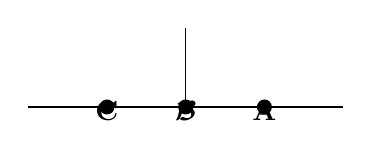
\begin{tikzpicture}
		\draw
				(2,0) -- (1,0) node[label=below:{\(\mat{A}\)}]{}
				-- (0,0)
				(-2,0) -- (-1,0) node[label=below:{\(\mat{C}\)}]{}
				-- (0,0)
				(0,0) node[label=below:{\(\tensor{B}\)}]{} -- (0,1)
			;
		\end{tikzpicture}
		\caption{Three-way tensor train.}
	\end{subfigure}~
%	\begin{subfigure}[t]{0.45\textwidth}
%		\begin{tikzpicture}
%		\draw
%				(2,0) -- (1,0) node[label=below:{\(\mat{C}\)}]{}
%				-- (0,0)
%				(-2,0) -- (-1,0) node[label=below:{\(\mat{A}\)}]{}
%				-- (0,0)
%				(0,0) node[label=below:{\(\tensor{B}\)}]{} -- (0,1)
%				-- (0,1) node[label=right:{\(\mat{C}\)}]{} -- (0,2)
%			;
%		\end{tikzpicture}
%		\caption{Three-way Tucker decomposition.}
%		\label{fig:tuckertnd}
%	\end{subfigure}\\
	\begin{subfigure}[t]{0.45\textwidth}
		\begin{tikzpicture}
		\draw
				(-2,0) -- (-1,0) node{}
				-- (0,0) node{} -- (0,1)
				(-1,0) -- (-1, 1)
				(0,0) -- (0,1)
				(0,0) -- (1,0)
				
				(2,0) -- (3,0) node{}
				-- (4,0)
				(3,0) -- (3, 1)
			;
		\path (1,0) -- node[auto=false, draw=none, fill=none] {\ldots} (2,0);
		\end{tikzpicture}
		\caption{General Tensor Train}
	\end{subfigure}
	\caption{Diagrams of the Tensor Train decomposition.}
	\label{fig:tttnds}
\end{figure}

\section{Bilinear Product}
Computing a bilinear product between two vectors and a tensor in the TT-decomposition does not
have quite such an efficient form as the CP-decomposition. Primarily this is due to the presence
of the three-way tensor \(\tensor{B}\), which means we are still eventually computing a full
tensor product, simply with a smaller tensor. We denote the product as
\begin{equation} \label{eq:tt_bilin}
	\vec{z} = \vec{x}^\mathsf{T}\mat{A}\tensor{B}\mat{C}\vec{y}.
\end{equation} For a specific index this has the form
\begin{align} \label{eq:tt_bilin_index}
	z_j &= \tran{\vec{x}}\vec{A}\mat{B}_{\midbullet j \midbullet}\mat{C}\vec{y}
		= \sum_{i}^{n_1}\sum_{k}^{n_3}
		\sum_{\alpha_1}^{r_1}
		\sum_{\alpha_2}^{r_2}A_{i\alpha_1}B_{\alpha_1j\alpha_2}C_{\alpha_2k}x_iy_k.
\end{align}

Eq.~\eqref{eq:tt_bilin} provides a clear intuition about what the TT-decomposition is doing in 
the three-way case.
Matrices \(\mat{A}\) and \(\mat{C}\) project the inputs into a new (potentially smaller) space
where the bilinear product is carried out with \(\tensor{B}\) ensuring the result has been pushed
back to the appropriate size.

\section{Gradients}
The gradient of \(\vec{z}\) with respect to \(\mat{A}\) has entries of the form:
\begin{align}
	\frac{\partial z_j}{\partial A_{lm}} 
	    &= \sum_{k}^{n_3}
		\sum_{\alpha_2}^{r_2}B_{m j\alpha_2}C_{\alpha_2k}x_ly_k
		= x_l \cdot \left(\tran{\vec{B}_{mj\midbullet}}\mat{C}\vec{y}\right). \\
\intertext{The components of the gradient with respect to \(\mat{C}\) have a similar form:}
	\frac{\partial z_j}{\partial C_{lm}} 
		&= \sum_{i}^{n_1}
		\sum_{\alpha_1}^{r_1}A_{i\alpha_1}B_{\alpha_1jl}x_iy_m 
		= y_m \cdot \left(\tran{\vec{B}_{\midbullet jl}}\mat{A}\vec{x}\right). \\
\intertext{While the gradient of the elements of \(\tensor{B}\) behave similarly
	to the CP-decomposition:}
	\frac{\partial z_j}{\partial B_{lmn}} 
		&= \sum_{i}^{n_1}\sum_{k}^{n_3}
		A_{il}C_{nk}x_iy_k. \\
\end{align}
This is very similar to the CP-decomposition. Again the central
object -- which is in this case a three-way tensor -- has highly redundant gradients, although it
is not clear what effect this may have on learning.


\section{Comparison with CP}
It is worth comparing the Tensor Train decomposition with the CP decomposition. In the three-way
case we find they are very closely related but that the CP has some key advantages. 

\subsection{Equivalence}
One condition for the tensor-train to be equivalent to the CP-decomposition is if the central
tensor in the TT-decomposition has diagonal, square slices. Intuitively this reduces the tensor
product to a matrix product. 

\begin{prop}
The rank \(R\) CP-decomposition of a tensor \(\tensor{X} = [\mat{A},\mat{B},\mat{C}]_{CP}\) is
equivalent to a TT-decomposition \([\mat{A}', \tensor{B}', \mat{C}']_{TT}\) with both ranks
equal to \(R\) and \(\tensor{B}'_{ijk} = 0\) except where \(i=k\).
\end{prop}
\begin{proof}
Consider the slices of \(\tensor{X} \in \mathbb{R}^{n_1 \times n_2 \times n_3}\) formed by fixing the
second index and allowing the first and third to vary. If 
\(\tensor{X} = [\mat{A}, \mat{B}, \mat{C}]_{CP}\) then these slices can be expressed concisely as
\begin{equation} \label{eq:cp-slice}
	\mat{X}_{\midbullet j \midbullet} = \mat{A}\diag({\mat{B}_{j\midbullet}})\tran{\mat{C}}
\end{equation} where \(\diag(\vec{v})\) denotes the matrix with vector \(\vec{v}\) along the
leading diagonal and zero elsewhere. 
It is clear the the diagonal matrix must then have shape
\(R \times R\) so the result has the expected shape \(n_1 \times n_3\). We also verify this gives us
the appropriate expression for a single element of the tensor:
\begin{align}
	X_{ijk} &= \left(\mat{A}\diag({\mat{B}_{j\midbullet}})\tran{\mat{C}}\right)_{ik} 
		    = \sum_{\alpha=1}^R A_{i\alpha} \cdot
		    	\left(\sum_{\beta=1}^{R} \diag(B_{j\midbullet})_{\alpha\beta} C_{k\beta}\right) 
			= \sum_{\alpha=1}^R A_{i\alpha} B_{j\alpha} C_{k\alpha}
\end{align} where the last step follows from diagonality.

We now construct a TT-decomposition \(\tensor{X} = [\mat{A}', \tensor{B}', \mat{C}']_{TT}\)
of the same tensor. The ranks of the decomposition will be \(r_1 = r_2 = R\) for \(R\) the rank
of the corresponding CP-decomposition.
Let \(\mat{A}' = \mat{A}\) and \(\mat{C}' = \tran{\mat{C}}\). Construct tensor \(\tensor{B}'\)
by
\begin{equation}
	B_{ijk}' = \begin{cases}
		B_{ij} & \text{if}\; i = k \\
		0    & \text{otherwise}.
	\end{cases}
\end{equation}

An expression for the central slices of \(\tensor{X}\) in terms of its TT-decomposition which
follows from the element-wise definition is
\begin{align}
	\mat{X}_{\midbullet j \midbullet} &= \mat{A}'\mat{B}_{\midbullet j \midbullet}'\mat{C}'\\
	&= \mat{A}\diag(B_{j\midbullet})\tran{\mat{C}}.
\end{align}
\end{proof}

%As is demonstrated in figure~\ref{fig:tuckertnd} the Tucker decomposition is very similar to the 
%tensor-train in the three-way case. For brevity we refrain from presenting the full Tucker
%decomposition -- it suffices to note that it has matrices for all three dimensions rather than
%just two. In order to convert the Tucker decomposition to the tensor-train, it is enough to multiply
%the additional matrix with the central tensor. For that reason, we prefer the simpler tensor-train.

\subsection{Space Requirements}
The number of stored coefficients for a rank \(R\) CP-decomposed tensor of size 
\(I \times J \times K\) will be \(RI + RJ + RK\). Explicitly storing the tensor would require
\(IJK\) numbers to be stored. To illustrate the significance of this, consider the case when
the tensor being decomposed has all dimensions and rank of equal size. Denoting the size as
\(I\), then the explicit tensor will have an \(I^3\) storage requirement while the decomposed
tensor needs only \(3RI\), a remarkable reduction.

For a TT decomposition with ranks \((R_1, R_2)\) and dimensions \(I \times J \times K\) we need
\(R_1I + R_1JR_2 + R_2K\) storage. If both ranks are equal, this becomes \(RI + R^2J + RK\), which
is quadratic in the rank. As the ranks have to be integers, this gives us less ability to fine-tune the
number of parameters in the decomposition as changing the ranks by small amounts may have large
implications on the size of the decomposition.

The CP decomposition is clearly the most appealing in this regard. Not only does it only require a
single hyper-parameter to control the size, the fact that it grows linearly in that hyper-parameter
makes it much more amenable to adjustment.

\subsection{Experiments}
In this section we detail experiments comparing the two decompositions.

\subsubsection{Random Bilinear Products}\label{sec:randbilin}
\paragraph{Goal.}
The aim for this experiment is to compare the two decompositions. There are two scenarios to
investigate: learning a decomposed tensor when the tensor has the same structure as the data and
learning a decomposed tensor when it can only approximate the underlying structure. 

\paragraph{Experiment Details.}
This test uses the following procedure: generate a fixed random tensor \(\tensor{T}\)
in the chosen decomposition with rank \(r_T\). Then generate a second tensor \(\tensor{W}\) 
with rank \(r_W\). At each stage \(t\) generate a pair of random input vectors \(\vec{x}_t\) and
\(\vec{y}_t\) and compute the bilinear products 
\(\vec{z}_tt = \vec{x}_t^\mathsf{T}\tensor{T}\vec{y}_t\) and 
\(\hat{\vec{z}}_t = \vec{x}_t^\mathsf{T}\tensor{W}\vec{y}_t\). Finally update the parameters of
\(\tensor{W}\) to minimise the mean squared error between \(\vec{z}^t\) and \(\hat{\vec{z}}^t\)
using stochastic gradient descent. In this way we hope to learn an approximation to 
\(\tensor{T}\) in a similar setting to what might be found inside a neural network.

We use a batch size of \(32\) and a fairly aggressive
 learning rate of \(0.1\).
Training continues for \(250,000\) parameter updates, although most of the tensors have stopped
making significant improvements by that time. In all tests the input vectors had elements drawn
from a uniform distribution over the range \([-1,1]\) while unless otherwise noted the elements of
the decomposition are drawn from a normal distribution with mean \(0\) and standard deviation
\(0.1\). We use the same random seed for each trial, which explains the similar patterns in the
TT-decompositions loss curves.

\paragraph{Results.}

\begin{figure}[ht]
\centering
\begin{subfigure}[t]{0.45\textwidth}
	\includegraphics[width=\textwidth]{tensors/cp100cpapprox}
	\caption{Attempting to approximate by directly learning factor matrices representing a 
		CP-decomposition of various ranks}
	\label{fig:cpcpapprox}
\end{subfigure}
\hfill
\begin{subfigure}[t]{0.45\textwidth}
	\includegraphics[width=\textwidth]{tensors/cp100ttapprox}
	\caption{Attempting to approximate by directly learning a TT-decomposition of various ranks}
	\label{fig:cpttapprox}
\end{subfigure}
\caption{Results for learning direct approximations of a CP-rank 100 tensor.}
 \label{fig:cpapprox}
\end{figure}

\begin{figure}[ht]
\centering
\begin{subfigure}[t]{0.45\textwidth}
	\includegraphics[width=\textwidth]{tensors/tt16cpapprox}
	\caption{Attempting to approximate by directly learning a 
		CP-decomposition of various ranks}
	\label{fig:ttcpapprox}
\end{subfigure}
\hfill
\begin{subfigure}[t]{0.45\textwidth}
	\includegraphics[width=\textwidth]{tensors/tt16ttapprox}
	\caption{Attempting to approximate by directly learning a TT-decomposition of various ranks}
	\label{fig:ttttapprox}
\end{subfigure}
\caption{Results for learning direct approximations of a tt-rank 16 tensor.}
\label{fig:ttapprox}
\end{figure}
The results of attempting to approximate a (CP) rank 100 tensor with dimensions 
\(100 \times 100 \times 100\) (which has 30,000 independent coefficients) 
are shown in figure~\ref{fig:cpapprox}.
The CP-decomposition is able to perfectly represent it when the rank is high enough,
but usefully it is able to converge on reasonable approximations when it can not
represent the full tensor.
The TT-decomposition struggled, both in stability during training and final error.
While we might expect the CP-decomposition to better represent another CP-decomposition due to
the shared structure, it is remarkable how difficult the TT-decomposition was to
train.
In general we see that the quality of the approximation drops consistently with the
number of parameters in the approximator, which is to be expected.

The experiment was repeated with the target tensor expressed is a TT-decomposition with ranks
\(r_1 = r_2 = 16\) (28,800 coefficients). Results can be seen in figure~\ref{fig:ttapprox}.
As should be expected, the TT-decomposition performed better. In particular a TT-decomposition
matching the rank of the target tensor reached a very low error extraordinarily quickly,
performing much better than the CP-decomposition under the same conditions.

These results imply both decompositions are potentially useful. The CP-decomposition learns
 reasonable approximations even when it does not necessarily reflect the
structure of the underlying problem. The TT-decomposition struggles in this situation,
but when the problem is structured more favourably it takes greater advantage.

\subsubsection{Learning to multiply}
\paragraph{Goal.}
Learning bilinear functions provides a way to linearly approximate functions of two variables.
A motivating example of such a function is element-wise multiplication, also known as the Hadamard
product. In this section we investigate briefly the ability of the two decompositions to model
such a product. We are particularly concerned with this as generalising this operation provides
significant motivation for the current investigation.

\paragraph{Experiment Details.}
Learning exact element-wise products is a special case and can clearly be done with the 
CP-decomposition without sacrificing parameter reduction. The question that remains is how closely
a given decomposition can approximate an element-wise product, especially if there is some kind of
helpful latent structure in the inputs to exploit. We test this by inducing a random structure
on the inputs.

This is performed identically to the experiments in section~\ref{sec:randbilin}
except that that rather than generating a random tensor to provide the targets for training,
we simply multiply element-wise the input vectors. We also simplify slightly by drawing the
input vectors from \(\{0,1\}\) with equal probability
(element-wise multiply in this sense corresponds to a bitwise AND). 
Again the squared error loss is used, although
a momentum term (with coefficient 0.9) was found to greatly assist learning.
For a further test, the target
output has a fixed permutation applied which removes the diagonal structure from the target but
should still be a straightforward task. For this task we would
expect that the CP-decomposition drastically outperforms the TT-decomposition.

For a more realistic test we introduce a random structure to the input vectors. This is done by
creating smaller vectors and expanding them to the appropriate size by copying the
elements to random positions. The mapping of positions is fixed for the duration of a training
run. We then experiment with varying the size of these smaller vectors and hence varying the
degree of correlation between elements
while keeping the rank of the decomposition being trained fixed. Here we have fewer
preconceptions regarding the relative performance of the decompositions -- by introducing structure
and reducing the complexity of the target relationship we would hope to see both decompositions making
good progress.

\paragraph{Results.}
The results are shown in figure~\ref{fig:multiply-ff}
and affirm our expectations. 
The CP-decomposition is able to consistently reduce error as rank increases
 while the TT-decomposition appears to struggle. Permuting the indices did not make any
 difference to the relative performance.

When there is significant structure to the inputs, the
TT decomposition is notably worse. One hypothesis is that the CP decomposition simply represents
higher rank tensors with the same number of parameters and that this is is what allows to better
represent more complex structures. This is shown in the other results -- the rank 1 decompositions
achieve similar performance regardless of the decomposition.

\begin{figure}
	\begin{subfigure}[t]{0.45\textwidth}
		\includegraphics[width=\textwidth]{tensors/multiply-cp-mom}
		\caption{Learning curves for CP-decompositions learning element-wise multiplication}
	\end{subfigure}
	\hfill
	\begin{subfigure}[t]{0.45\textwidth}
		\includegraphics[width=\textwidth]{tensors/multiply-tt-mom}
		\caption{Learning curves for TT-decompositions learning element-wise multiplication}
	\end{subfigure}
	\caption{Training error for various rank decompositions on the element-wise multiplication
	task.}
	\label{fig:multiply-ff}
\end{figure}


\begin{figure}
	\begin{subfigure}[t]{0.45\textwidth}
		\includegraphics[width=\textwidth]{tensors/permute-cp-mom}
		\caption{Learning curves for CP-decompositions learning permuted 
		element-wise multiplication}
	\end{subfigure}
	~
	\begin{subfigure}[t]{0.45\textwidth}
		\includegraphics[width=\textwidth]{tensors/permute-tt-mom}
		\caption{Learning curves for TT-decompositions learning permuted
		 element-wise multiplication}
	\end{subfigure}
	\caption[Permuted element-wise multiplication results]{Training error for various rank decompositions on the permuted
	element-wise multiplication
	task.}
	\label{fig:permute-multiply-ff}
\end{figure} 

\begin{figure}
	\begin{subfigure}[t]{0.45\textwidth}
		\includegraphics[width=\textwidth]{tensors/correlatecp50-mom}
		\caption{Learning curves for a rank 50 CP-decomposition.}
	\end{subfigure}
	\hfill
	\begin{subfigure}[t]{0.45\textwidth}
		\includegraphics[width=\textwidth]{tensors/correlatett11-mom}
		\caption{Learning curves for a rank 11 TT-decomposition.}
	\end{subfigure}
	\caption{Training error for two decompositions learning element-wise multiplication with
	 varying amounts of structure.}
	\label{fig:correlate-multiply}
\end{figure}

\section{Conclusion}
In the three-way case, it is clear the the CP-decomposition is preferable. Theoretically it should
be able to maintain its expressive power even at low-rank (and therefore with few parameters).
Empirically this indeed seems to be the case. 

\chapter{Additional Tables}
\begin{table}
\centering
\begin{tabu} to 0.5\linewidth {|r|l|}
\hline 
\textit{Description} & \textit{Example} \\
\hline
scalar & \(a\) \\
vector & \(\vec{b}\) \\
matrix & \(\mat{C}\) \\
higher order tensor & \(\tensor{D}\) \\
element of vector (scalar) & \(b_i\) \\
element of matrix (scalar) & \(C_{ij}\) \\
element of 3-tensor (scalar) & \(D_{ijk}\) \\
row of matrix (vector) & \(\vec{C}_{i\midbullet}\) \\
column of matrix (vector) & \(\vec{C}_{\midbullet i}\)\\
\textit{fiber} of 3-tensor (vector) & \(\vec{D}_{\midbullet jk}\)\\
\textit{slice} of 3-tensor (matrix) & \(\mat{D}_{\midbullet\midbullet k}\)\\
\hline
\end{tabu}
\caption{Example of notation for tensors.}
\label{tab:notation}
\end{table}

This chapter contains additional tables which were omitted from the main text due to space
requirements. They are not essential to the main text, but provide illustrative examples.

\chapter{Additional Figures}
This chapter contains a number of figures omitted from the main text because the relationships
they reveal are very close to earlier figures.

\section{Synthetic Tasks}
\subsection{Addition}
\subsubsection{Task}
Figure~\ref{fig:additionpics} shows an example input sequence for the addition task discussed in 
section~\ref{sec:addition}. This was generated by training a TGU with 2 hidden units and rank 1
 to solve the
task on sequences of length 50. We show the input to the network and the values of the network's
hidden states.

\begin{figure}
\centering
\begin{tabu} to \textwidth {rX}
states: & \includegraphics[width=0.75\textwidth]{exps/addition/states0} \\
inputs: & \includegraphics[width=0.75\textwidth]{exps/addition/inputs0}
\end{tabu}

\caption[Addition example]{Example of inputs and states for a network solving the addition task.
Images are greyscale, with lower values darker. The bottom line is the input to the network while the
top row is its hidden states -- clearly it accumulates the appropriate input in a single hidden unit.}
\label{fig:additionpics}
\end{figure}

\subsubsection{Results}
Figure~\ref{fig:addsmall} shows results for the addition task on the smaller of the sequences attempted.
Results are very similar to those at sequence length 750.
\begin{figure}
\centering
\begin{subfigure}[t]{0.75\textwidth}
\includegraphics[width=\textwidth]{exps/addition/sl250}
\caption{Sequence length 250.}
\label{fig:add250}
\end{subfigure}

\begin{subfigure}[t]{0.75\textwidth}
\includegraphics[width=\textwidth]{exps/addition/sl500}
\caption{Sequence length 500.}
\label{fig:add500}
\end{subfigure}
\caption{Addition results, smaller sequences.}
\label{fig:addsmall}
\end{figure}

\subsection{Variable Binding} \label{sec:vbinddata}
\subsubsection{Task}

\begin{figure}
\centering
	\begin{tabu} to \textwidth {XX}
		Input & Target \\
		\includegraphics[width=0.45\textwidth, interpolate=false]{exps/vbind/100x1input} & 
		\includegraphics[width=0.45\textwidth, interpolate=false]{exps/vbind/100x1target} \\
		\includegraphics[width=0.45\textwidth, interpolate=false]{exps/vbind/100x2input} & 
		\includegraphics[width=0.45\textwidth, interpolate=false]{exps/vbind/100x2target} \\
		\includegraphics[width=0.45\textwidth, interpolate=false]{exps/vbind/100x3input} & 
		\includegraphics[width=0.45\textwidth, interpolate=false]{exps/vbind/100x3target} \\
	\end{tabu}
	\caption[Example instances of variable binding]{Example input/target pairs for the three
	different variable binding tasks. All have length 100, with 8 bit patterns -- all that differs
	is the number of patterns the network may have to remember at once.}
	\label{fig:vbinddata}
\end{figure}

\begin{figure}
\centering
	\begin{tabu} to \textwidth {XX}
		Input & Output \\
		\includegraphics[width=0.45\textwidth, interpolate=false]{exps/vbind/100x1tguinput} & 
		\includegraphics[width=0.45\textwidth, interpolate=false]{exps/vbind/100x1tguoutput} \\
		\includegraphics[width=0.45\textwidth, interpolate=false]{exps/vbind/100x2tguinput} & 
		\includegraphics[width=0.45\textwidth, interpolate=false]{exps/vbind/100x2tguoutput} \\
		\includegraphics[width=0.45\textwidth, interpolate=false]{exps/vbind/100x3tguinput} & 
		\includegraphics[width=0.45\textwidth, interpolate=false]{exps/vbind/100x3tguoutput} \\
	\end{tabu}
	\caption[Example successful outputs for variable binding]{Outputs from TGU models that that
	achieved good results.}
	\label{fig:vbindcorrect}
\end{figure}

\begin{figure}
\centering
	\begin{tabu} to \textwidth {XX}
		Input & Output \\
		\includegraphics[width=0.45\textwidth, interpolate=false]{exps/vbind/100x1gruinput} & 
		\includegraphics[width=0.45\textwidth, interpolate=false]{exps/vbind/100x1gruoutput} \\
		\includegraphics[width=0.45\textwidth, interpolate=false]{exps/vbind/100x2gruinput} & 
		\includegraphics[width=0.45\textwidth, interpolate=false]{exps/vbind/100x2gruoutput} \\
		\includegraphics[width=0.45\textwidth, interpolate=false]{exps/vbind/100x3gruinput} & 
		\includegraphics[width=0.45\textwidth, interpolate=false]{exps/vbind/100x3gruoutput} \\
	\end{tabu}
	\caption[Example of baseline for variable binding]{Output from GRUs demonstrating the baseline
	behaviour -- the timing is correct but the output is not related to the input.}
	\label{fig:vbindfail}
\end{figure}

Figures~\ref{fig:vbinddata}, \ref{fig:vbindcorrect} and \ref{fig:vbindfail} all show examples of
the inputs and outputs for the variable binding task. Including the outputs of a successful network
and an network that failed to progress beyond the baseline.

\section{Real Data}

\subsection{Polyphonic Music}
The sizes of the models used are reported in table~\ref{tab:jsbsizes}.


\begin{table}
\begin{tabu} to \linewidth {r||c|c|c|c}
\hline
Model & \multicolumn{4}{|c}{hidden units/rank (parameters)} \\
\hline
Vanilla & \multicolumn{4}{|c}{96  (19927)} \\
LSTM & \multicolumn{4}{|c}{44 (20075)} \\
GRU & \multicolumn{4}{|c}{52 (19763)} \\
\hline
GMR & 95/1 (19870) & 71/35 (19872) & 58/58 (19775) & 45/90 (20125) \\
GMR-C & 349/1 (20005) & 106/52 (20142) & 76/76 (20119) & 53/106 (20248) \\
TGU &  80/1 (20030) & 63/31 (20156) &  53/53 (20248) & 41/82 (19817) \\
TGU-C &  176/1 (20000) & 88/44 (20075) & 66/66 (19855) & 48/96 (20071)\\
\hline
\end{tabu}
\caption[Model sizes for polyphonic music task]{Size of models for polyphonic music
modelling. Architectures with -C appended have the bias matrices combined with the
decomposition. Parameters are reported for inputs of size \(54\) as per the JSB dataset.
Rank is only reported if applicable.}
\label{tab:jsbsizes}
\end{table}

\chapter{Additional Proofs}
There are a number of useful facts which are used throughout the document. Here we provide
proofs of those which are not necessarily obvious.

\section{Element-wise multiplication by bilinear product}
This is a useful point about the structure of a tensor implementing element-wise
multiplication.
\begin{prop} [Identity Tensor] \label{prop:identity}
	\(\tensor{H} \in \mathbb{R}^{N \times N \times N}\) such that
\begin{align}
\vec{x}^\mathsf{T}\tensor{H}\vec{y} = \vec{x} \odot \vec{y}, 
&&\forall \vec{x},\vec{y} \in \mathbb{R}^{N}
\end{align} implies
\begin{equation}
	H_{ijk} = \begin{cases}
		1 & \text{if}\;\;i = j = k \\
		0 & \text{otherwise.}
	\end{cases}
\end{equation}

\end{prop}
\begin{proof}
We prove briefly, by inspecting one component of the result. Let 
\(\vec{z} = \vec{x}^\mathsf{T}\tensor{H}\vec{y}\). Then
\begin{align}
	z_j &= \vec{x}^\mathsf{T}\mat{H}_{\midbullet j \midbullet}\vec{y} \\
		&= \sum_i^N\sum_k^N x_iH_{ijk}y_k
\end{align}
If \(z_j = x_jy_j\) as in the elementwise product, then it is clear we want \(H_{ijk}\) to be 
1 if \(i=j=k\). Further, if we ensure \(H_{ijk}\) is 0 when this is not the case we can see that
the rest of the terms in the sums will disappear.
\end{proof}

\chapter{Initialization}\label{A:init}
RNNs can be sensitive to initialisation, especially with regard to learning long
time dependencies \autocite{Le2015}. It has been suggested that a good initialisation should
have eigenvalues on or inside the complex unit circle \autocite{Zilly2016, Mikolov2015} which
would suggest initialising to an orthogonal or orthonormal matrix as per. \autocite{Henaff2016}.

Figure~\ref{fig:inits} shows some simplified simulations to illustrate the effect of
different methods of initialisation in conjunction with different forms of gated recurrence. They are
simulated with no non-linearity and a single input at the first time step sampled from a unit
normal. If gate values are required, they are sampled uniformly in \([0,1]\). We then simply
run the recurrence over the hidden state for a number of time steps plotting each cell's state
as a grayscale value. This makes it quite clear whether the initialisation preserves the variance
of the original input by observing the patterns it makes. Significant periodicities are
good as they indicate the network has plenty of temporal information to latch onto during
training. If most of the state is uniform grey it would suggest that the state vanishes
or explodes.

We show three possible procedures: random normal (mean 0, standard deviation 0.01), spectral
normalised and orthonormal. The spectral normalised matrix is a random normal matrix that
has been divided by a fraction of its leading singular value. This ensures the spectral
radius of the matrix is slightly greater than one. To generate a random orthonormal matrix
we generate a random matrix from a normal distribution, compute its QR decomposition and use the
Q.

\begin{figure}
\centering
\begin{subfigure}[t]{0.3\textwidth}
\includegraphics[width=\textwidth]{appendix/init/vanillanormal}
\caption{Vanilla transition, normal initialisation.}
\end{subfigure}\hfill
\begin{subfigure}[t]{0.3\textwidth}
\includegraphics[width=\textwidth]{appendix/init/lstmnormal}
\caption{Forget gate transition, normal initialisation.}
\end{subfigure}\hfill
\begin{subfigure}[t]{0.3\textwidth}
\includegraphics[width=\textwidth]{appendix/init/grunormal}
\caption{Convex gate transition, normal initialisation.}
\end{subfigure}\\

\begin{subfigure}[t]{0.3\textwidth}
\includegraphics[width=\textwidth]{appendix/init/vanillaspec}
\caption{Vanilla transition, spectral normalised initialisation.}
\end{subfigure}\hfill
\begin{subfigure}[t]{0.3\textwidth}
\includegraphics[width=\textwidth]{appendix/init/lstmspec}
\caption{Forget gate transition, spectral normalised initialisation.}
\end{subfigure}\hfill
\begin{subfigure}[t]{0.3\textwidth}
\includegraphics[width=\textwidth]{appendix/init/gruspec}
\caption{Convex gate transition, spectral normalised initialisation.}
\end{subfigure}\\

\begin{subfigure}[t]{0.3\textwidth}
\includegraphics[width=\textwidth]{appendix/init/vanillaorth}
\caption{Vanilla transition, orthonormal initialisation.}
\end{subfigure}\hfill
\begin{subfigure}[t]{0.3\textwidth}
\includegraphics[width=\textwidth]{appendix/init/lstmorth}
\caption{Forget gate transition, orthonormal initialisation.}
\end{subfigure}\hfill
\begin{subfigure}[t]{0.3\textwidth}
\includegraphics[width=\textwidth]{appendix/init/gruorth}
\caption{Convex gate transition, orthonormal initialisation.}
\end{subfigure}\\

\caption[Simulated RNN states from various initialisations]{Example simulations of RNN states from different initialisation. Images are
independently normalised, with darker values being more negative and lighter more positive.}
\label{fig:inits}
\end{figure}

Results are in figure~\ref{fig:inits}. Clearly initialising from a normal distribution is
insufficient. The spectral normalisation also tends to explode (note that often the initial
random state is no longer visible, this is because the degree of normalisation required
to display the final states). Correspondingly we prefer the orthonormal initialisation
throughout this report, although we note that with Vanilla RNNs which preserve information
nearly perfectly from this initialisation we occasionally had to scale the entire matrix down
by a constant factor to avoid exploding early in training.


\chapter{Algorithms for Synthetic Tasks}

\section{Addition}\label{sec:additionpseudo}
Data for the addition task can be generated by algorithm~\ref{alg:additiondata}. This algorithm
produces a single item, it could also be done in batches with slight adjustments.

\begin{algorithm}
	\KwIn{Integer \(T\)}
	\KwOut{Problem instance \((\vec{x}_1, \vec{x}_2, \ldots, \vec{x}_T), y\)}
	\BlankLine
	Sample integer \(i \sim U[1, (T/2)-1]\)\;
	Sample integer \(j \sim U[T/2, T]\)\;
	\(y \gets 0\)\;
	\For{\(t \in \{1, \ldots, T\}\)}{
		Sample float \(x_{t1} \sim U[0,1]\)\;
		\If{\(t = i\) or \(t = j\)} {
			\(y \gets y + x_{t1}\)\;
			\(x_{t2} \gets 1\)\;
		} \Else {
			\(x_{t2} \gets 0\)\;
		}
	}
	\KwRet{\((\vec{x}_1, \vec{x}_2, \ldots, \vec{x}_T), y\)}
	\caption{Generating data for addition task}
	\label{alg:additiondata}
\end{algorithm}

\section{Variable binding}\label{sec:vbindpseudo}
Algorithm~\ref{alg:vbinddata} shows how to generate a single data item for this task. This algorithm
is indicative only, there are ways to be more efficient especially if it has to be implemented as a
computation graph, for example in Tensorflow.

\begin{algorithm}
	\KwIn{Integers \(T, D, N\)}
	\KwOut{Problem instance \((\vec{x}_1,\ldots,\vec{x}_T), (\vec{y}_1,\ldots,\vec{y}_T)\)}
	\BlankLine
	intialise \((\vec{x}_1,\ldots,\vec{x}_T), (\vec{y}_1,\ldots,\vec{y}_T)\) to zeros\;
	\For{\(i \in \{1, \ldots, N\}\)} {
		Sample integer \(j \sim U[1, (T/2)-1]\) \tcc*{start position}
		Sample integer \(k \sim U[j+1, T]\) \tcc*{end position}
		\(\vec{z} \gets\) random \(D\) bit binary pattern\;
		\(\vec{y}_{k+1} \gets \vec{z}\)\;
		Set first \(D\) bits of \(\vec{x}_{i+1}\) to \(\vec{z}\)\;
		\For(set label bits){\(l \in \{j,\ldots,k\}\)}{
			\({x}_{l, D+i} \gets 1\)\;
		}
	}
	\KwRet{\((\vec{x}_1,\ldots,\vec{x}_T), (\vec{y}_1,\ldots,\vec{y}_T)\)}
	
	\caption{Generating data for variable binding}
	\label{alg:vbinddata}
\end{algorithm}
%TC:endignore

%%%%%%%%%%%%%%%%%%%%%%%%%%%%%%%%%%%%%%%%%%%%%%%%%%%%%%%

\backmatter

%%%%%%%%%%%%%%%%%%%%%%%%%%%%%%%%%%%%%%%%%%%%%%%%%%%%%%%


%\bibliographystyle{ieeetr}
%\bibliographystyle{acm}
%\bibliography{sample}
\printbibliography

\end{document}
